\documentclass[aspectratio=169]{beamer}
\usepackage{german}
\usepackage[utf8]{inputenc} %for windows
\usepackage[T1]{fontenc}
\usepackage{textcomp}
\usepackage{gensymb}
\usepackage{graphicx}
\usepackage{tikz}
\usepackage{pgfplots}
\usepackage{xcolor}
\usepackage{siunitx}
\usepackage{listings}
\usepackage{caption, subcaption}
\usepackage{verbatim}
\usepackage{eso-pic} %to draw on top right corner
\usepackage{xpatch}
\usepackage{multicol}

%define hsr colors
\definecolor{hsrBlue}{RGB}{000,101,163}
\definecolor{hsrHematite}{RGB}{110,028,080}
\definecolor{hsrLakeGreen}{RGB}{084,140,134}
\definecolor{hsrReed}{RGB}{123,105,081}
\definecolor{hsrPetrol}{RGB}{000,115,141}
\definecolor{hsrBasswood}{RGB}{186,189,093}
\definecolor{hsrGray}{RGB}{198,199,200}
\definecolor{hsrBlack}{RGB}{026,023,027}

%design & color
\usetheme[width=2.2cm]{PaloAlto}
\usecolortheme{beaver}
\useinnertheme{circles}
\usefonttheme[onlymath]{serif}
\setbeamercolor{section in sidebar}{fg=hsrBlack}
\setbeamercolor{itemize item}{fg=hsrBlue}
\setbeamercolor{itemize subitem}{fg=hsrLakeGreen}
\setbeamercolor{item projected}{fg=white,bg=hsrBlack}
\setbeamercolor{title in sidebar}{fg=hsrBlack}
\setbeamercolor{author in sidebar}{fg=hsrBlue} 
\setbeamercolor{caption name}{fg=hsrBlue}
\setbeamercolor*{title}{fg=hsrBlue}
\setbeamercolor{frametitle}{fg=hsrBlue, bg=hsrGray!15!white}
\setbeamercolor{sidebar}{bg=hsrGray!15!white}
\setbeamercolor{logo}{bg=hsrGray!0!white}

%disable navigation symbols
\beamertemplatenavigationsymbolsempty
%slide numbers
\setbeamertemplate{footline}[frame number]

%used for drawing n(r)-Area
\definecolor{lGray}{gray}{0.8}
\definecolor{llGray}{gray}{0.9}
\usepgfplotslibrary{fillbetween}
\usetikzlibrary{fadings}

\definecolor{listinggray}{gray}{0.9}
\definecolor{lbcolor}{rgb}{0.97,0.97,0.97}
\definecolor{lightGray}{gray}{0.1}

\definecolor{cOrange}{HTML}{996633}
\definecolor{clOrange}{HTML}{DBB48D}
\definecolor{cBlue}{HTML}{336699}
\definecolor{clBlue}{HTML}{A0BCD8}
\definecolor{cGreen}{HTML}{339966}
\definecolor{clGreen}{HTML}{94D4B4}
\definecolor{cRed}{HTML}{993333}
\definecolor{clRed}{HTML}{D0B0B0}
\definecolor{cGray}{gray}{0.4}
\definecolor{clGray}{gray}{0.96}

\tikzset{>=stealth}

\newcommand{\eurobot}{$\text{Eurobot}^\text{open}$\ }

% ----- lstListings (C++ code with syntax highlighting) -----
\lstset{
	backgroundcolor=\color{lbcolor},
	xleftmargin=0.5cm,
	xrightmargin=0.5cm,
	tabsize=2,
	language=C++,
	captionpos=b,
	frame=none,
	numbers=none,
	numberstyle=\tiny,
	numbersep=5pt,
	breaklines=true,
	breakautoindent=true, 
	breakindent=20pt,
	breakatwhitespace=true,
	showstringspaces=false,
	%prebreak=\raisebox{0ex}[0ex][0ex]{\ensuremath{\color{cRed}\rhookswarrow}},
	postbreak=\raisebox{0ex}[0ex][0ex]{\ensuremath{\color{cRed}\lhookrightarrow\space}},
	basicstyle=\ttfamily,
	identifierstyle=\color{black},
	keywordstyle=\color{cRed},
	commentstyle=\color{cGreen},
	stringstyle=\color{cOrange},
	morekeywords={uint8_t, int8_t, uint16_t, int16_t, uint32_t, int32_t, bool},
	emph=[1]
	{
		%enum list
		connectionTimeout, ObtCom_msgTimeout,
		stIdle, stWaitForConnection, 
		evTimeout, evNewReq,evNewMsg, evReceivedReq, evReceivedAck, evReceivedErr, evReceivedAns, evNewXXX, evReceivedXXX, 
		msg, req, ans, ack, err, ObtCom_numIds,
		CAL_USR_INP_REQ, CAL_FIN,
		STOP_FORWARD, STOP_BACKWARD, STOP_DIR_AUTO, NO_LIMIT, FIX_DIR, TURN_FIRST
	},
	emphstyle=[1]{\color{cBlue}\textit},
	emph=[2]
	{
		%typedef list
		error_t,
		ObtCom_msgId_t,	ObtCom_msgReaction_t, ObtCom_ansReaction_t, ObtCom_reqReaction_t, ObtCom_msg_t, ObtCom_msgType_t,
		canCom_msg_t, canCom_moduleAddr_t, canCom_subId_t,
		senstime_t, sensmodule_t,
		posCtrl_way_t, posCtrl_stopDir_t, posCtrl_wayLimit_t, posCtrl_dest_t, pos_t
	},
	emphstyle=[2]{\color{cGreen!70!black}},
	emph=[3]
	{
		%function list
		main,
		canCom_init,
		fillStackWithPattern,
		encodeId, decodeId, ObtCom_validateMessage,
		display_registerNewSettingScreen, display_newSubMenuEntryToggle, display_newSubMenuEntrySelection, display_newSubMenuEntryButton, display_newSubMenuEntryText, display_newSubMenuEntryNumberInput, display_editEntryText, display_setVisibilitySubMenuEntry, display_drawScreen, display_isSubMenuActive,
		runTest, makeMenu, switchMode, getMode, toggleDebugMode, getDebugMode,setMaxSpeed, getMaxSpeed,
		calloc, malloc,
		cal_setError, cal_start, cal_stop, cal_off, cal_getMode, cal_reset,
		atan2,
		posCtrl_addDest, posCtrl_clearAllDests, posCtrl_getDest, posCtrl_secStop
	},
	emphstyle=[3]{\color{cBlue!60!black}},
}

%allow tikz animations
\tikzset{
	invisible/.style={opacity=0},
	visible on/.style={alt={#1{}{invisible}}},
	alt/.code args={<#1>#2#3}{%
		\alt<#1>{\pgfkeysalso{#2}}{\pgfkeysalso{#3}} % \pgfkeysalso doesn't change the path
	},
}

%use command const
\DeclareMathOperator{\const}{Konstant}

%title informations
\title[Eurobot] % (optional, only for long titles)
{Eurobot 2017 -- Moon Village}
\author[C. Angehrn \\M. Knöpfel \\T. Schneider] % (optional, for multiple authors)
{Cornel Angehrn \and Matthias Knöpfel \and Tibor Schneider}
\institute[hsr, imes] % (optional)
{
  HSR Hochschule für Technik Rapperswil \and
  IMES Institut für Mikroelektronik und Embedded Systems
}
%\date[KPT 2004] % (optional)
%{Conference on Presentation Techniques, 2004}
\subject{Embedded Systems}

%remove title and author from sidebar
\makeatletter
	\setbeamertemplate{sidebar \beamer@sidebarside}
	{
		\beamer@tempdim=\beamer@sidebarwidth
		\advance\beamer@tempdim by -6pt
		\insertverticalnavigation{\beamer@sidebarwidth}
		\vfill
		\ifx\beamer@sidebarside\beamer@lefttext
		\else
			\usebeamercolor{normal text}
			\llap{\usebeamertemplate***{navigation symbols}\hskip0.1cm}
			\vskip2pt
		\fi
	}
\setbeamertemplate{footline}
{
	\leavevmode%
	\hbox{%
		\begin{beamercolorbox}[wd=.333333\paperwidth,ht=2.25ex,dp=1ex,center]{title in head/foot}%
			\color{black} \insertshortauthor
		\end{beamercolorbox}%
		\begin{beamercolorbox}[wd=.333333\paperwidth,ht=2.25ex,dp=1ex,center]{title in head/foot}%
			\color{black} \insertshorttitle
		\end{beamercolorbox}%
		\begin{beamercolorbox}[wd=.333333\paperwidth,ht=2.25ex,dp=1ex,right]{title in head/foot}%
			\color{black} \insertshortdate{}\hspace*{2em}
			\color{black} \insertframenumber{} / \inserttotalframenumber\hspace*{2ex} 
	\end{beamercolorbox}}%
	\vskip0pt%
}
\patchcmd\beamer@@tmpl@frametitle{\insertframetitle}{\insertsection: \insertframetitle}{}{}
\makeatother


\begin{document}

  %titelseite
  \begingroup
  \makeatletter
  \setlength{\hoffset}{-.5\beamer@sidebarwidth}
  \makeatother
  \begin{frame}[plain]
  	\begin{figure}
	  	
\includegraphics[height=1.4cm]{../images/hsrImesLogo.jpg}
  	\end{figure}
  \titlepage 
  \end{frame}
	\endgroup
  
  %HSR-Logo auf allen Seiten ab hier
  \addtobeamertemplate{frametitle}{}{%
  \begin{tikzpicture}[remember picture,overlay]
  \node[anchor=north west,yshift=-8pt, xshift=-6pt, xshift=1.5pt] at (current page.north west) {
\includegraphics[height=0.8cm]{../images/HSR_Logo_A0.jpg}};
  \end{tikzpicture}} 

  %inhaltsverzeichnis
  %\frame{\frametitle{Inhaltsverzeichnis}\tableofcontents}
  
  %Einleitung
  \section{Einleitung}
\begin{frame}
	\frametitle{Einleitung}
	
	\begin{figure}
	   	\centering
	   	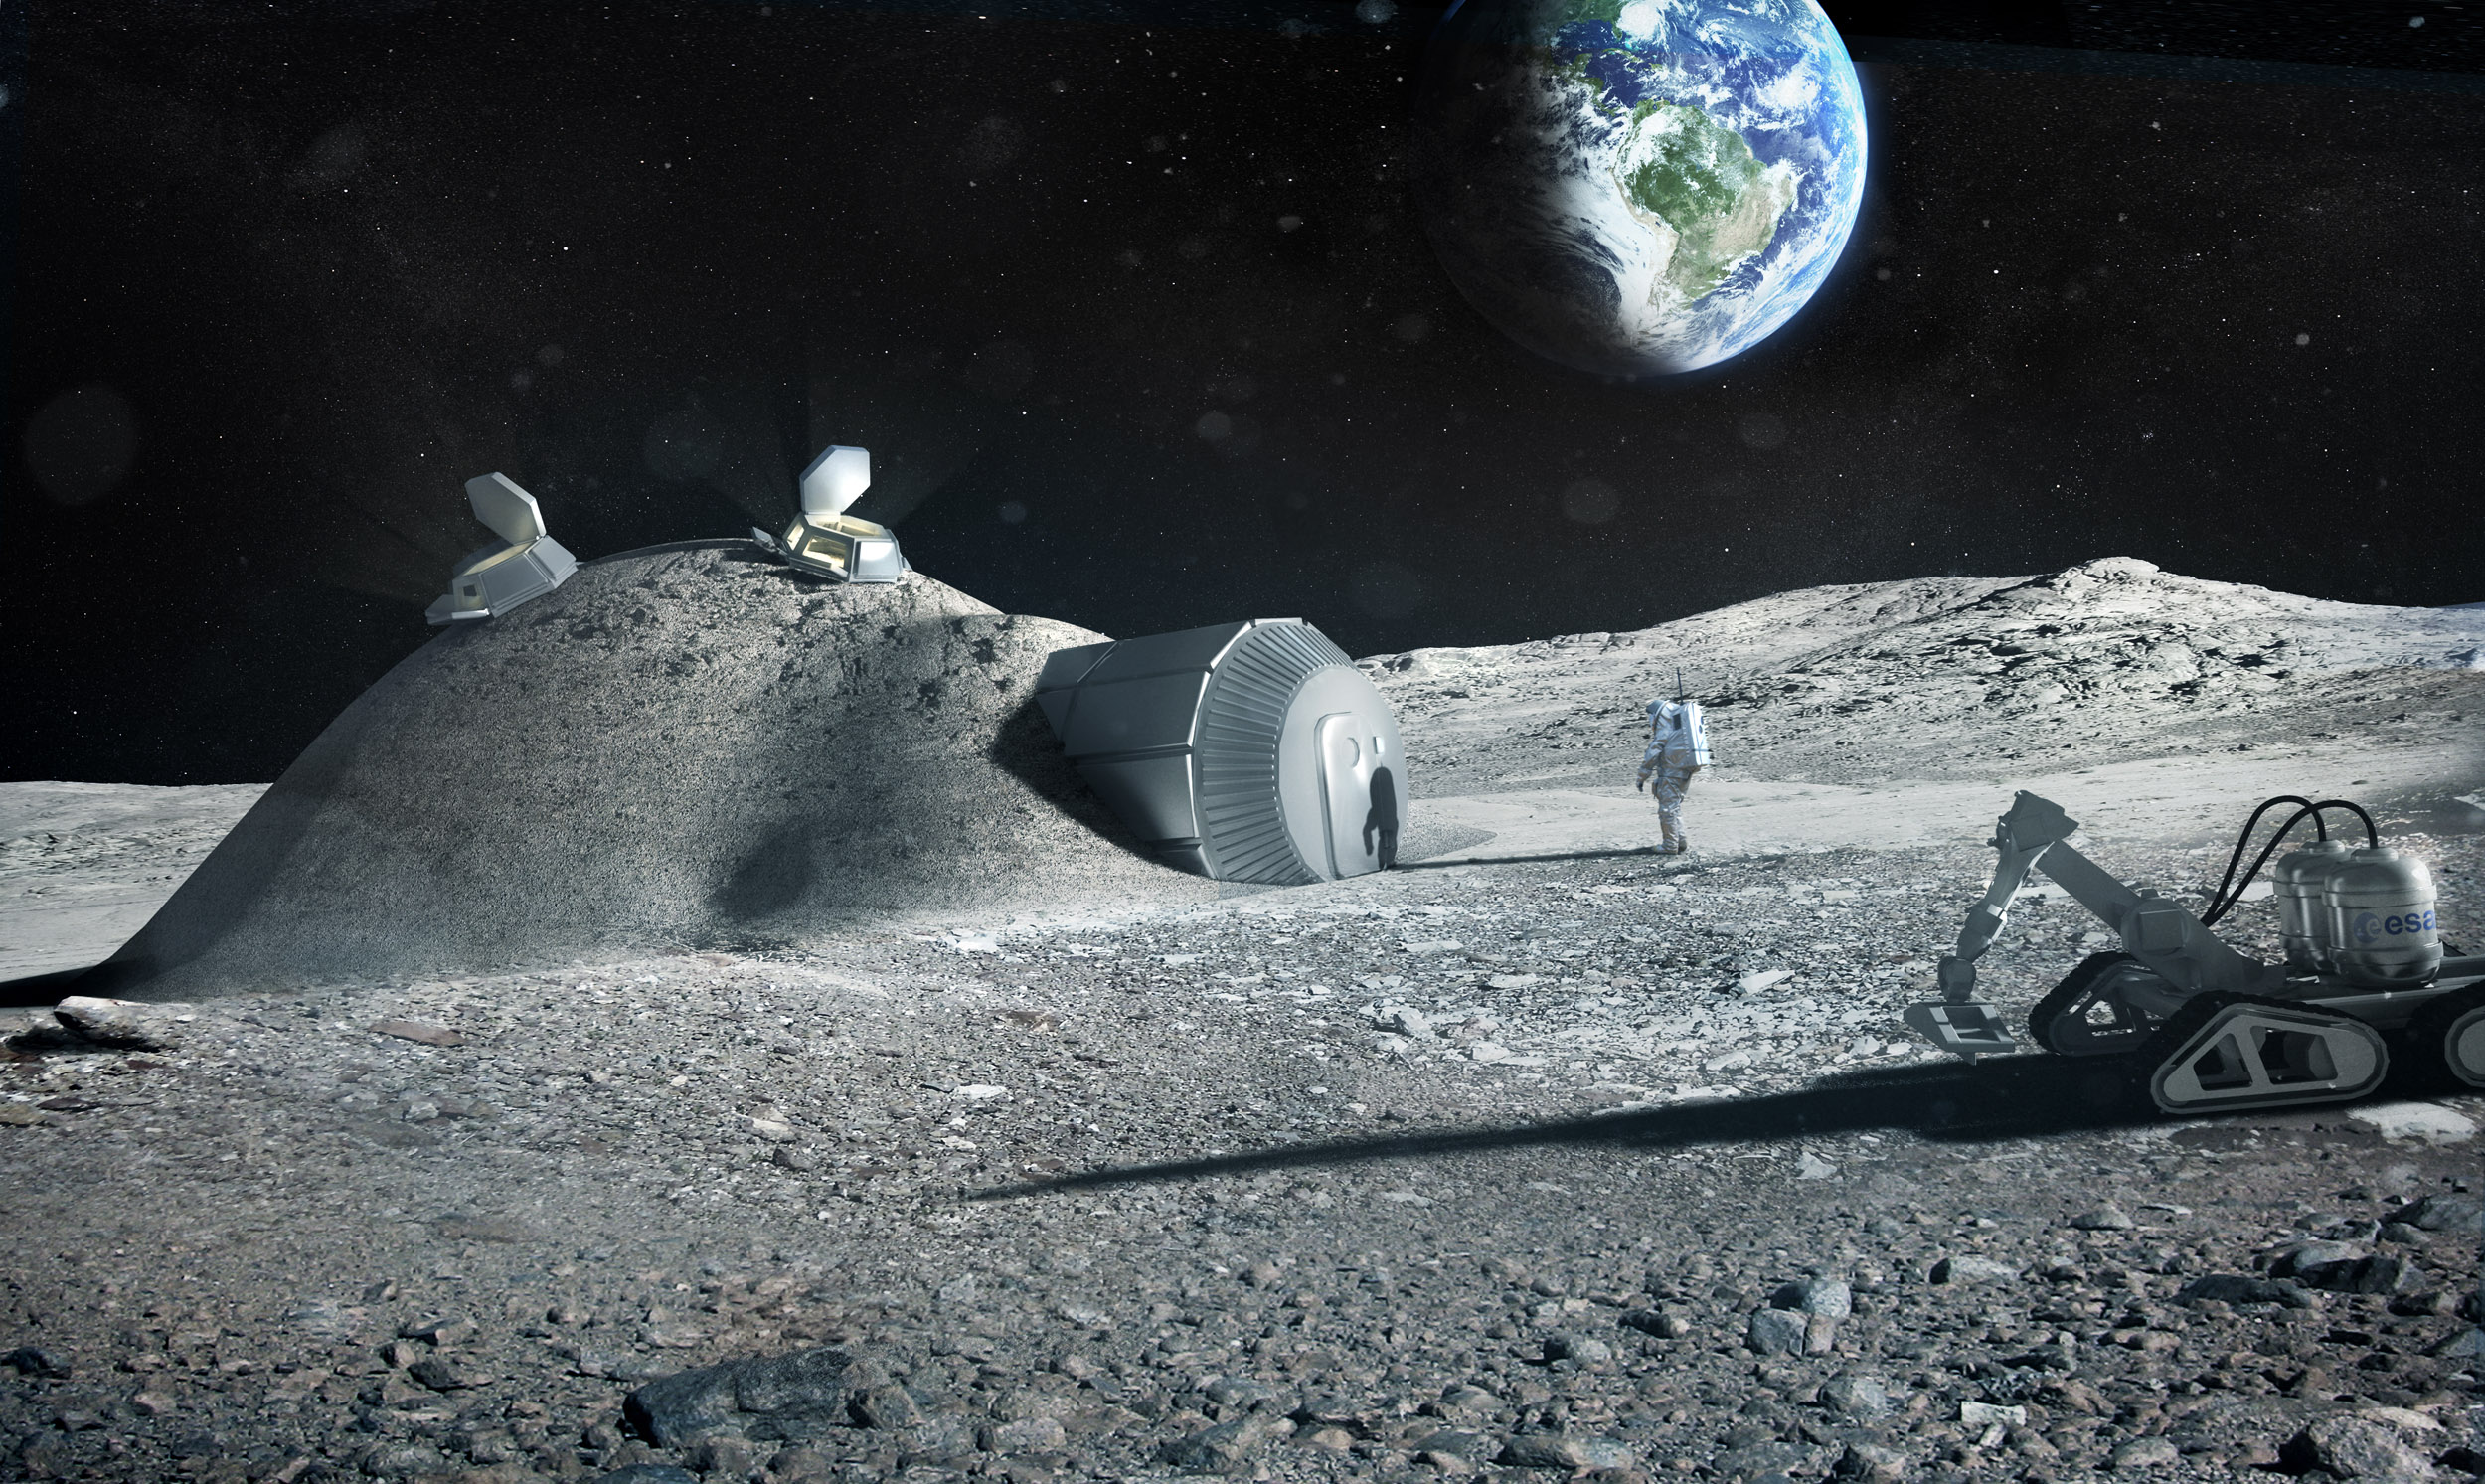
\includegraphics[height = 5cm]{../images/presentation/LunarBaseESA.jpg}
	   	\caption{Quelle: http://www.esa.int/spaceinimages/Images}
	\end{figure}
	
	%Lunar base aus 3D-Druck-Teilen und Mondgestein,
	%ESA (European Space Ageny)-Projekt,
	%Eurobot 2017-Wettbewerb unter diesem Moto

\end{frame} 

\begin{frame}
	\frametitle{Projektteam}
	
	\begin{figure}
		\begin{tikzpicture}[scale=0.5, transform shape]
		%Joel
		\def\xPos{2};	\def\yPos{1};
		\draw [draw=none, fill=hsrBlue] (\xPos - 2,\yPos - 4) rectangle (\xPos + 2,\yPos + 1);
		\draw [white] (\xPos,\yPos + 0.5) node{Joel Stolz};
		\draw [white] (\xPos,\yPos) node{\textbf{Mechanik}};
		\node[inner sep=0, outer sep=0, align=center] at (\xPos, \yPos - 2.2) {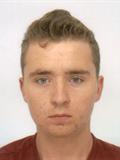
\includegraphics[height=3.5cm]{../images/Projektorganisation/joelStolz.jpg}};
		%Tibor
		\def\xPos{7};	\def\yPos{1};
		\draw [draw=none, fill=hsrBlue] (\xPos - 2,\yPos - 4) rectangle (\xPos + 2,\yPos + 1);
		\draw [white] (\xPos,\yPos + 0.5) node{Tibor Schneider};
		\draw [white] (\xPos,\yPos - 0) node{\textbf{Elektronik}};
		\node[inner sep=0, outer sep=0, align=center] at (\xPos, \yPos - 2.2) {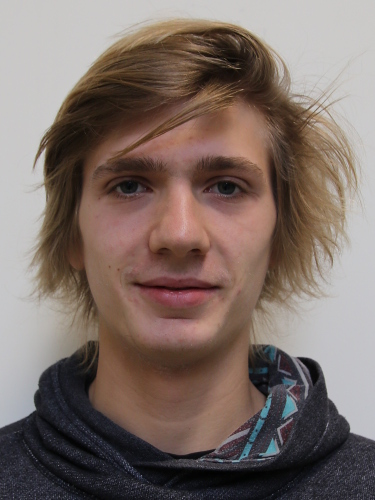
\includegraphics[height=3.5cm]{../images/Projektorganisation/tiborSchneider.jpg}};
		%cornel
		\def\xPos{12};	\def\yPos{1};
		\draw [draw=none, fill=hsrBlue] (\xPos - 2,\yPos - 4) rectangle (\xPos + 2,\yPos + 1);
		\draw [white] (\xPos,\yPos + 0.5) node{Cornel Angehrn};
		\draw [white] (\xPos,\yPos - 0) node{\textbf{Elektronik}};
		\node[inner sep=0, outer sep=0, align=center] at (\xPos, \yPos - 2.2) {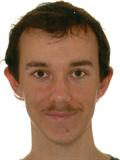
\includegraphics[height=3.5cm]{../images/Projektorganisation/cornelAngehrn.jpg}};
		%Matthias
		\def\xPos{17};	\def\yPos{1};
		\draw [draw=none, fill=hsrBlue] (\xPos - 2,\yPos - 4) rectangle (\xPos + 2,\yPos + 1);
		\draw [white] (\xPos,\yPos + 0.5) node{Matthias Knöpfel};
		\draw [white] (\xPos,\yPos - 0) node{\textbf{Elektronik}};
		\node[inner sep=0, outer sep=0, align=center] at (\xPos, \yPos - 2.2) {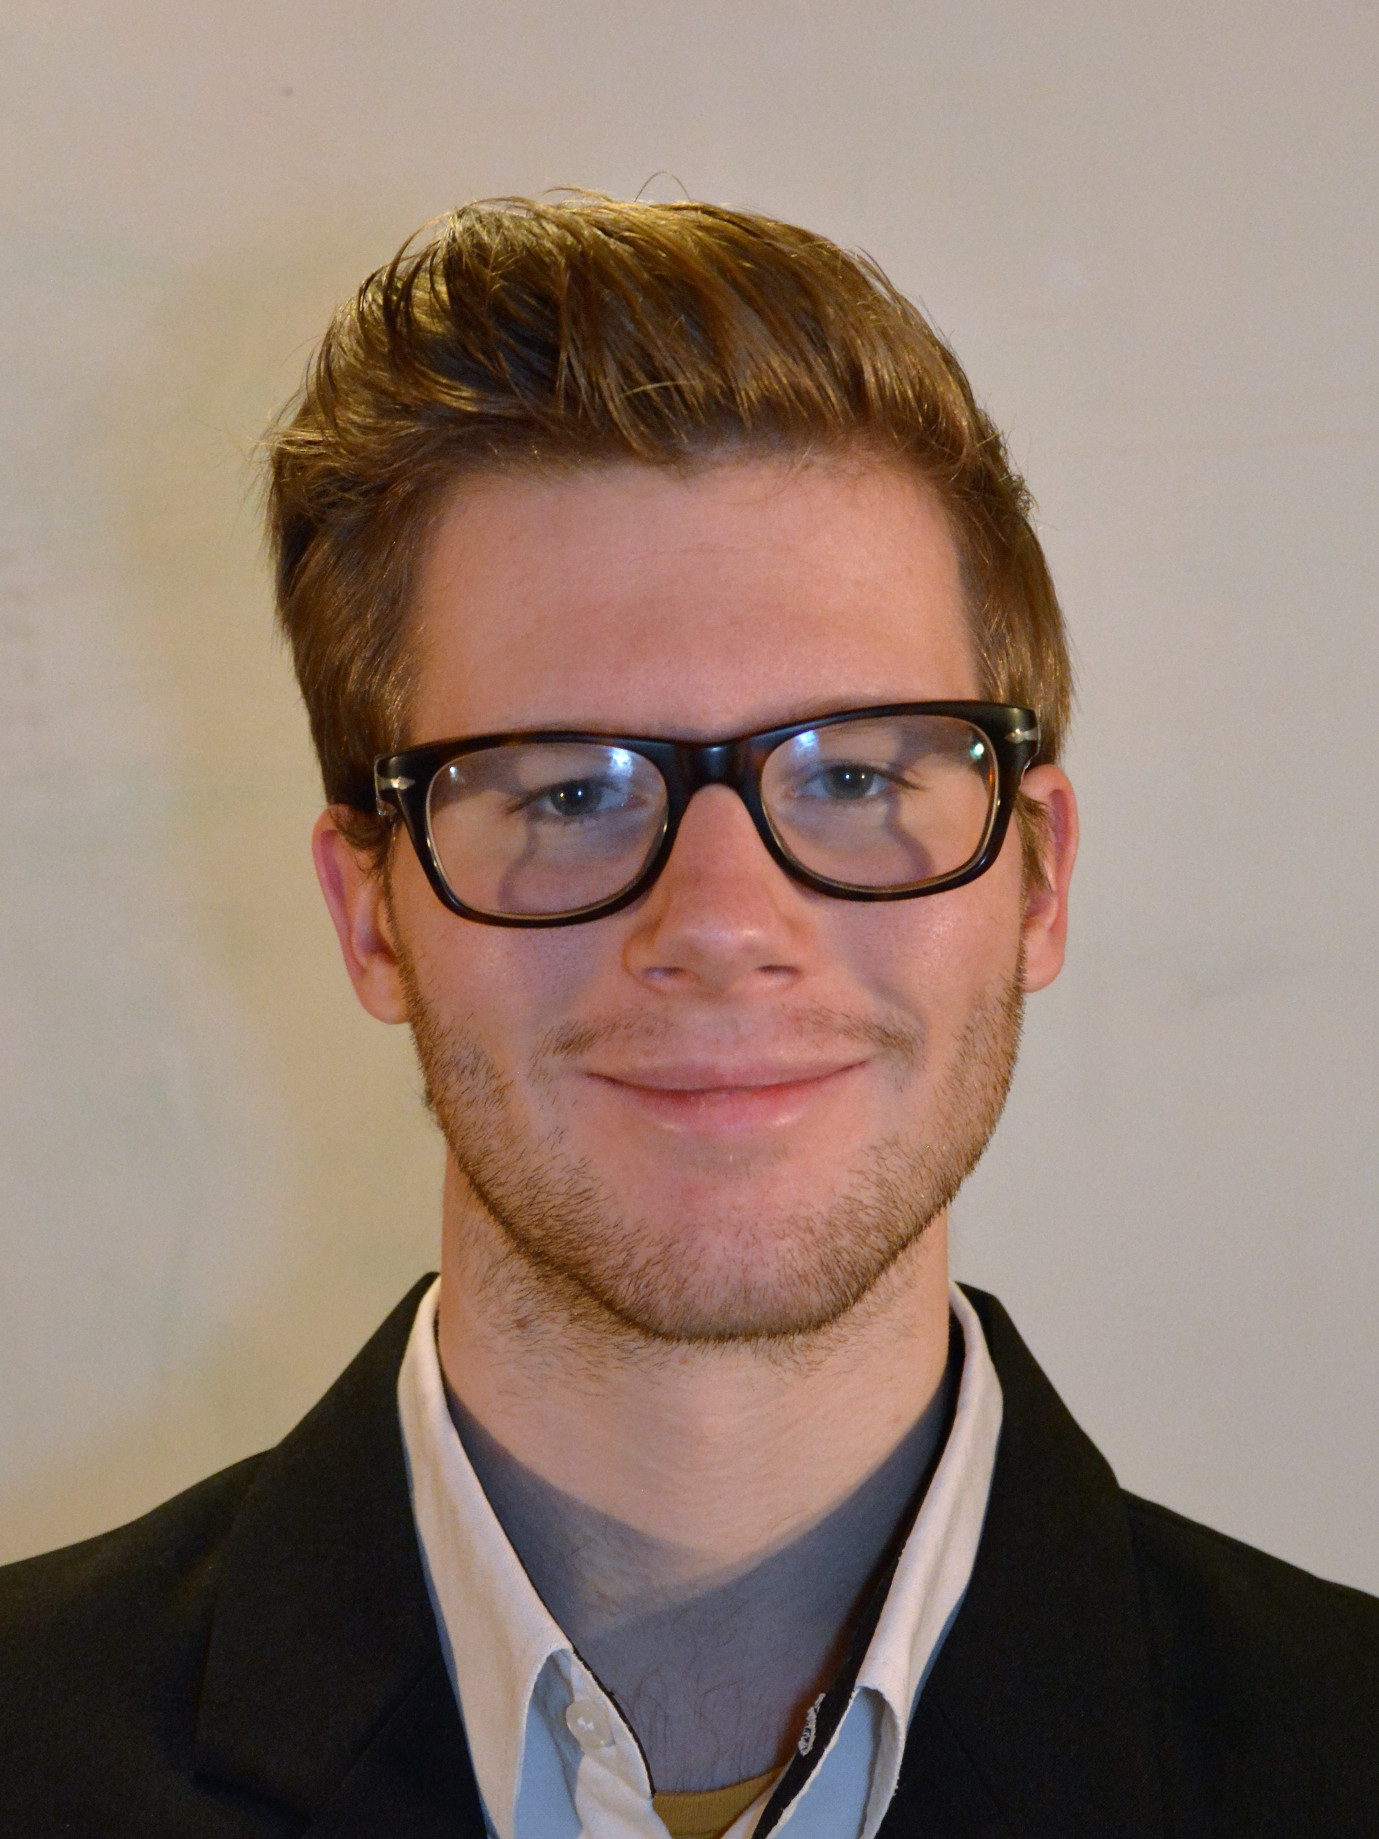
\includegraphics[height=3.5cm]{../images/Projektorganisation/matthiasKnoepfel.jpg}};
		%Petra
		\def\xPos{22};	\def\yPos{5};
		\draw [draw=none, fill=hsrBlue] (\xPos - 2,\yPos - 4) rectangle (\xPos + 2,\yPos + 1);
		\draw [white] (\xPos,\yPos + 0.5) node{Petra Freuler};
		\draw [white] (\xPos,\yPos - 0) node{\textbf{Projektleitung}};
		\node[inner sep=0, outer sep=0, align=center] at (\xPos, \yPos - 2.2) {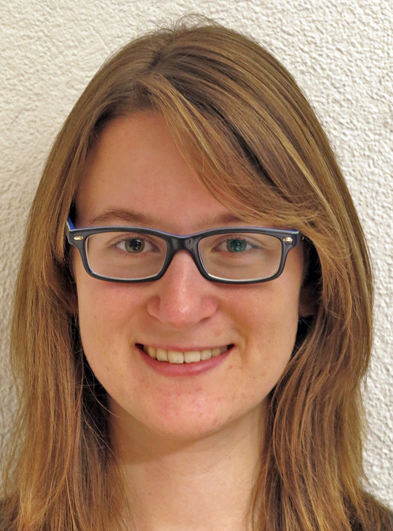
\includegraphics[height=3.5cm]{../images/Projektorganisation/petraFreuler.jpg}};
		%Wüst
		\def\xPos{2};	\def\yPos{8};
		\draw [draw=none, fill=hsrBlue] (\xPos - 2.5,\yPos - 1) rectangle (\xPos + 2.5,\yPos + 1);
		\draw [white] (\xPos,\yPos + 0.25) node{Prof. Theodor Wüst};
		\draw [white] (\xPos,\yPos - 0.25) node{\textbf{Betreuung Mechanik}};
		%Brändle
		\def\xPos{11};	\def\yPos{8};
		\draw [draw=none, fill=hsrBlue] (\xPos - 2.5,\yPos - 1) rectangle (\xPos + 2.5,\yPos + 1);
		\draw [white] (\xPos,\yPos + 0.5) node{Prof. Erwin Brändle};
		\draw [white] (\xPos,\yPos) node{\textbf{Auftraggeber}};
		\draw [white] (\xPos,\yPos - 0.5) node{\textbf{Betreuung Elektronik}};
		%Keller
		\def\xPos{17};	\def\yPos{8};
		\draw [draw=none, fill=hsrBlue] (\xPos - 2.5,\yPos - 1) rectangle (\xPos + 2.5,\yPos + 1);
		\draw [white] (\xPos,\yPos + 0.5) node{Prof. Daniel Keller};
		\draw [white] (\xPos,\yPos) node{\textbf{Betreuung}};
		\draw [white] (\xPos,\yPos - 0.5 ) node{\textbf{Projektleitung}};
		
		%connections
		\draw [thick] (2,2) -- (2,7) (2,3) -- (17,3) (7,2) -- (7,3) (12,2) -- (12,3) (17,2) -- (17,3) (11,3) -- (11,5) -- (20,5) (11,5) -- (11,7) (16,5) -- (17,5) -- (17,7);
		\end{tikzpicture}
	\end{figure}

\end{frame}

\begin{frame}
	\frametitle{Arbeitsaufteilung}
	
	\begin{itemize}
	   	\item Petra Freuler: Projektleitung %und Protokollführung
	   	\item Joel Stolz: Konstruktion, CAD	%gesamter Maschinenbauteil
	   	\item Cornel Angehrn: Gegnererkennung 
	   	\item Matthias Knöpfel: Fahrcontroller
	   	\item Tibor Schneider: Mainboard
	\end{itemize}
	
	\begin{itemize}
	   	\item Alle: Konzeptfindung, Machbarkeitstests
	\end{itemize}
	
	%Elektrotechnik: Dimensionieren und auswählen von Motoren, Sensoren und Beurteilung der Testergebnisse vorallem von elektrischer Seite (Vakuum/Saugnapf, Walze, Bälle fördern, ...)

\end{frame}
  
  %Spielbeschreibung
  \section{Spielbeschreibung}

\begin{frame}
	\frametitle{Tisch und Spielelemente}
	
\end{frame}

\begin{frame}
	\frametitle{Aufgaben und Punkte}
	
	\begin{figure}[H]
		\centering
		\begin{tabular}{|c|c|}
			\hline
			Ressourcen im Startfeld & 2 Punkte\\
			\hline
			\textit{Titanium Ores} in \textit{Cargo Bay} & 3 Punkte\\
			\hline
			\textit{Lunar Modules} in \textit{Moonbase} & 10 Punkte\\
			\hline
			\textit{Funny Action} & 20 Punkte\\
			\hline
			\hline
			\textit{Moon Rocks} & 0 Punkte\\
			\hline
			Bonus für aus dem Startfeld fahren & 15 Punkte\\
			\hline
			Strafe für unfaires und regelwidriges Verhalten & -20 Punkte\\
			\hline
		\end{tabular}	
	\end{figure}
\end{frame}

\begin{frame}
	\frametitle{Anforderungen an die Roboter}
	
	\begin{itemize}
		\item mechanische Abmessungen gemäss Reglement
		\item Roboter bewegen sich autonom
		\item keine Kollisionen mit Gegner
		\item keine gefährliche Techniken und Materialien (Pyrotechnik, starke Laser, ...)
	\end{itemize}
	
\end{frame}

\begin{frame}
	\frametitle{Wettbewerb}
	
	\begin{itemize}
		\item Homologation
	\end{itemize}
	\begin{itemize}
		\item 3 min Vorbereitungszeit
		\item 90 s Spiel
		\item \textit{Funny Action}
	\end{itemize}
	\begin{itemize}
		\item Finale \textit{Best-of-three}
	\end{itemize}
\end{frame}
  
  %Roboterfunktionen
  \section{Roboterfunktionen}

%todo vorschlag:

\begin{frame}
	\frametitle{Grosser Groboter}
	\vspace{-1.5em}
	\begin{figure}
		\begin{columns}[t]
			\column{0.5\textwidth}			
			\centering
			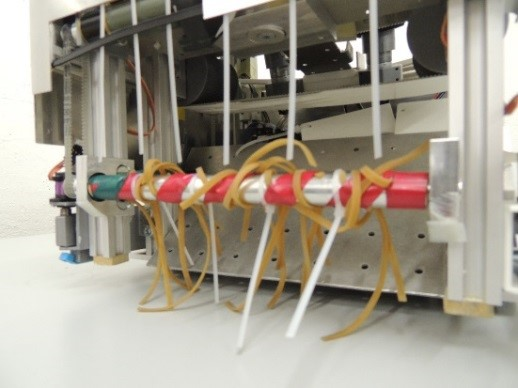
\includegraphics[width = 0.6\columnwidth]{../images/presentation/walze.jpg}\\\vspace{1em}
			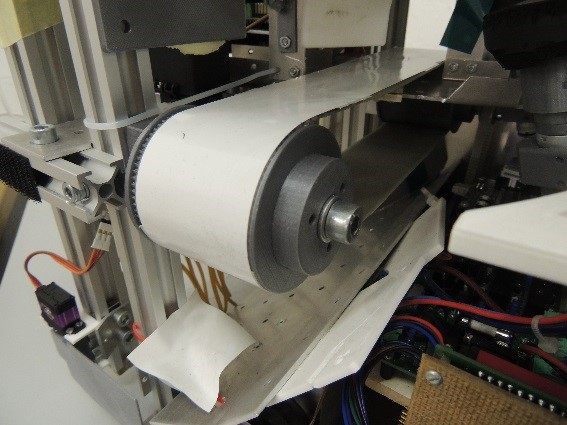
\includegraphics[width = 0.6\columnwidth]{../images/presentation/riemen.jpg}\\
			\column{0.5\textwidth}
			\centering
			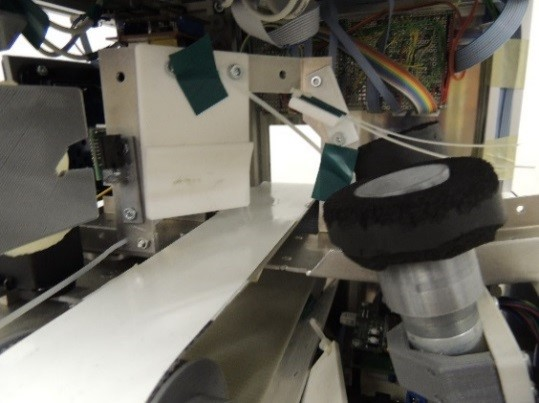
\includegraphics[width = 0.6\columnwidth]{../images/presentation/abstreifvorrichtung.jpg}\\\vspace{1em}
			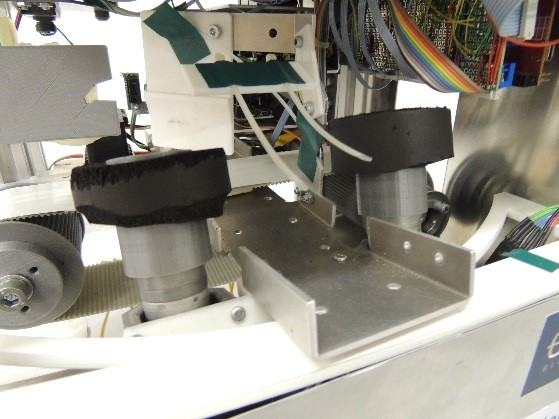
\includegraphics[width = 0.6\columnwidth]{../images/presentation/schussmechanismus.jpg}\\		
		\end{columns}
	\end{figure}
\end{frame}


\begin{frame}
	\frametitle{Kleiner Groboter}
	\vspace{-1.5em}
	\begin{figure}
		\begin{columns}[t]
			\column{0.5\textwidth}			
			\centering
			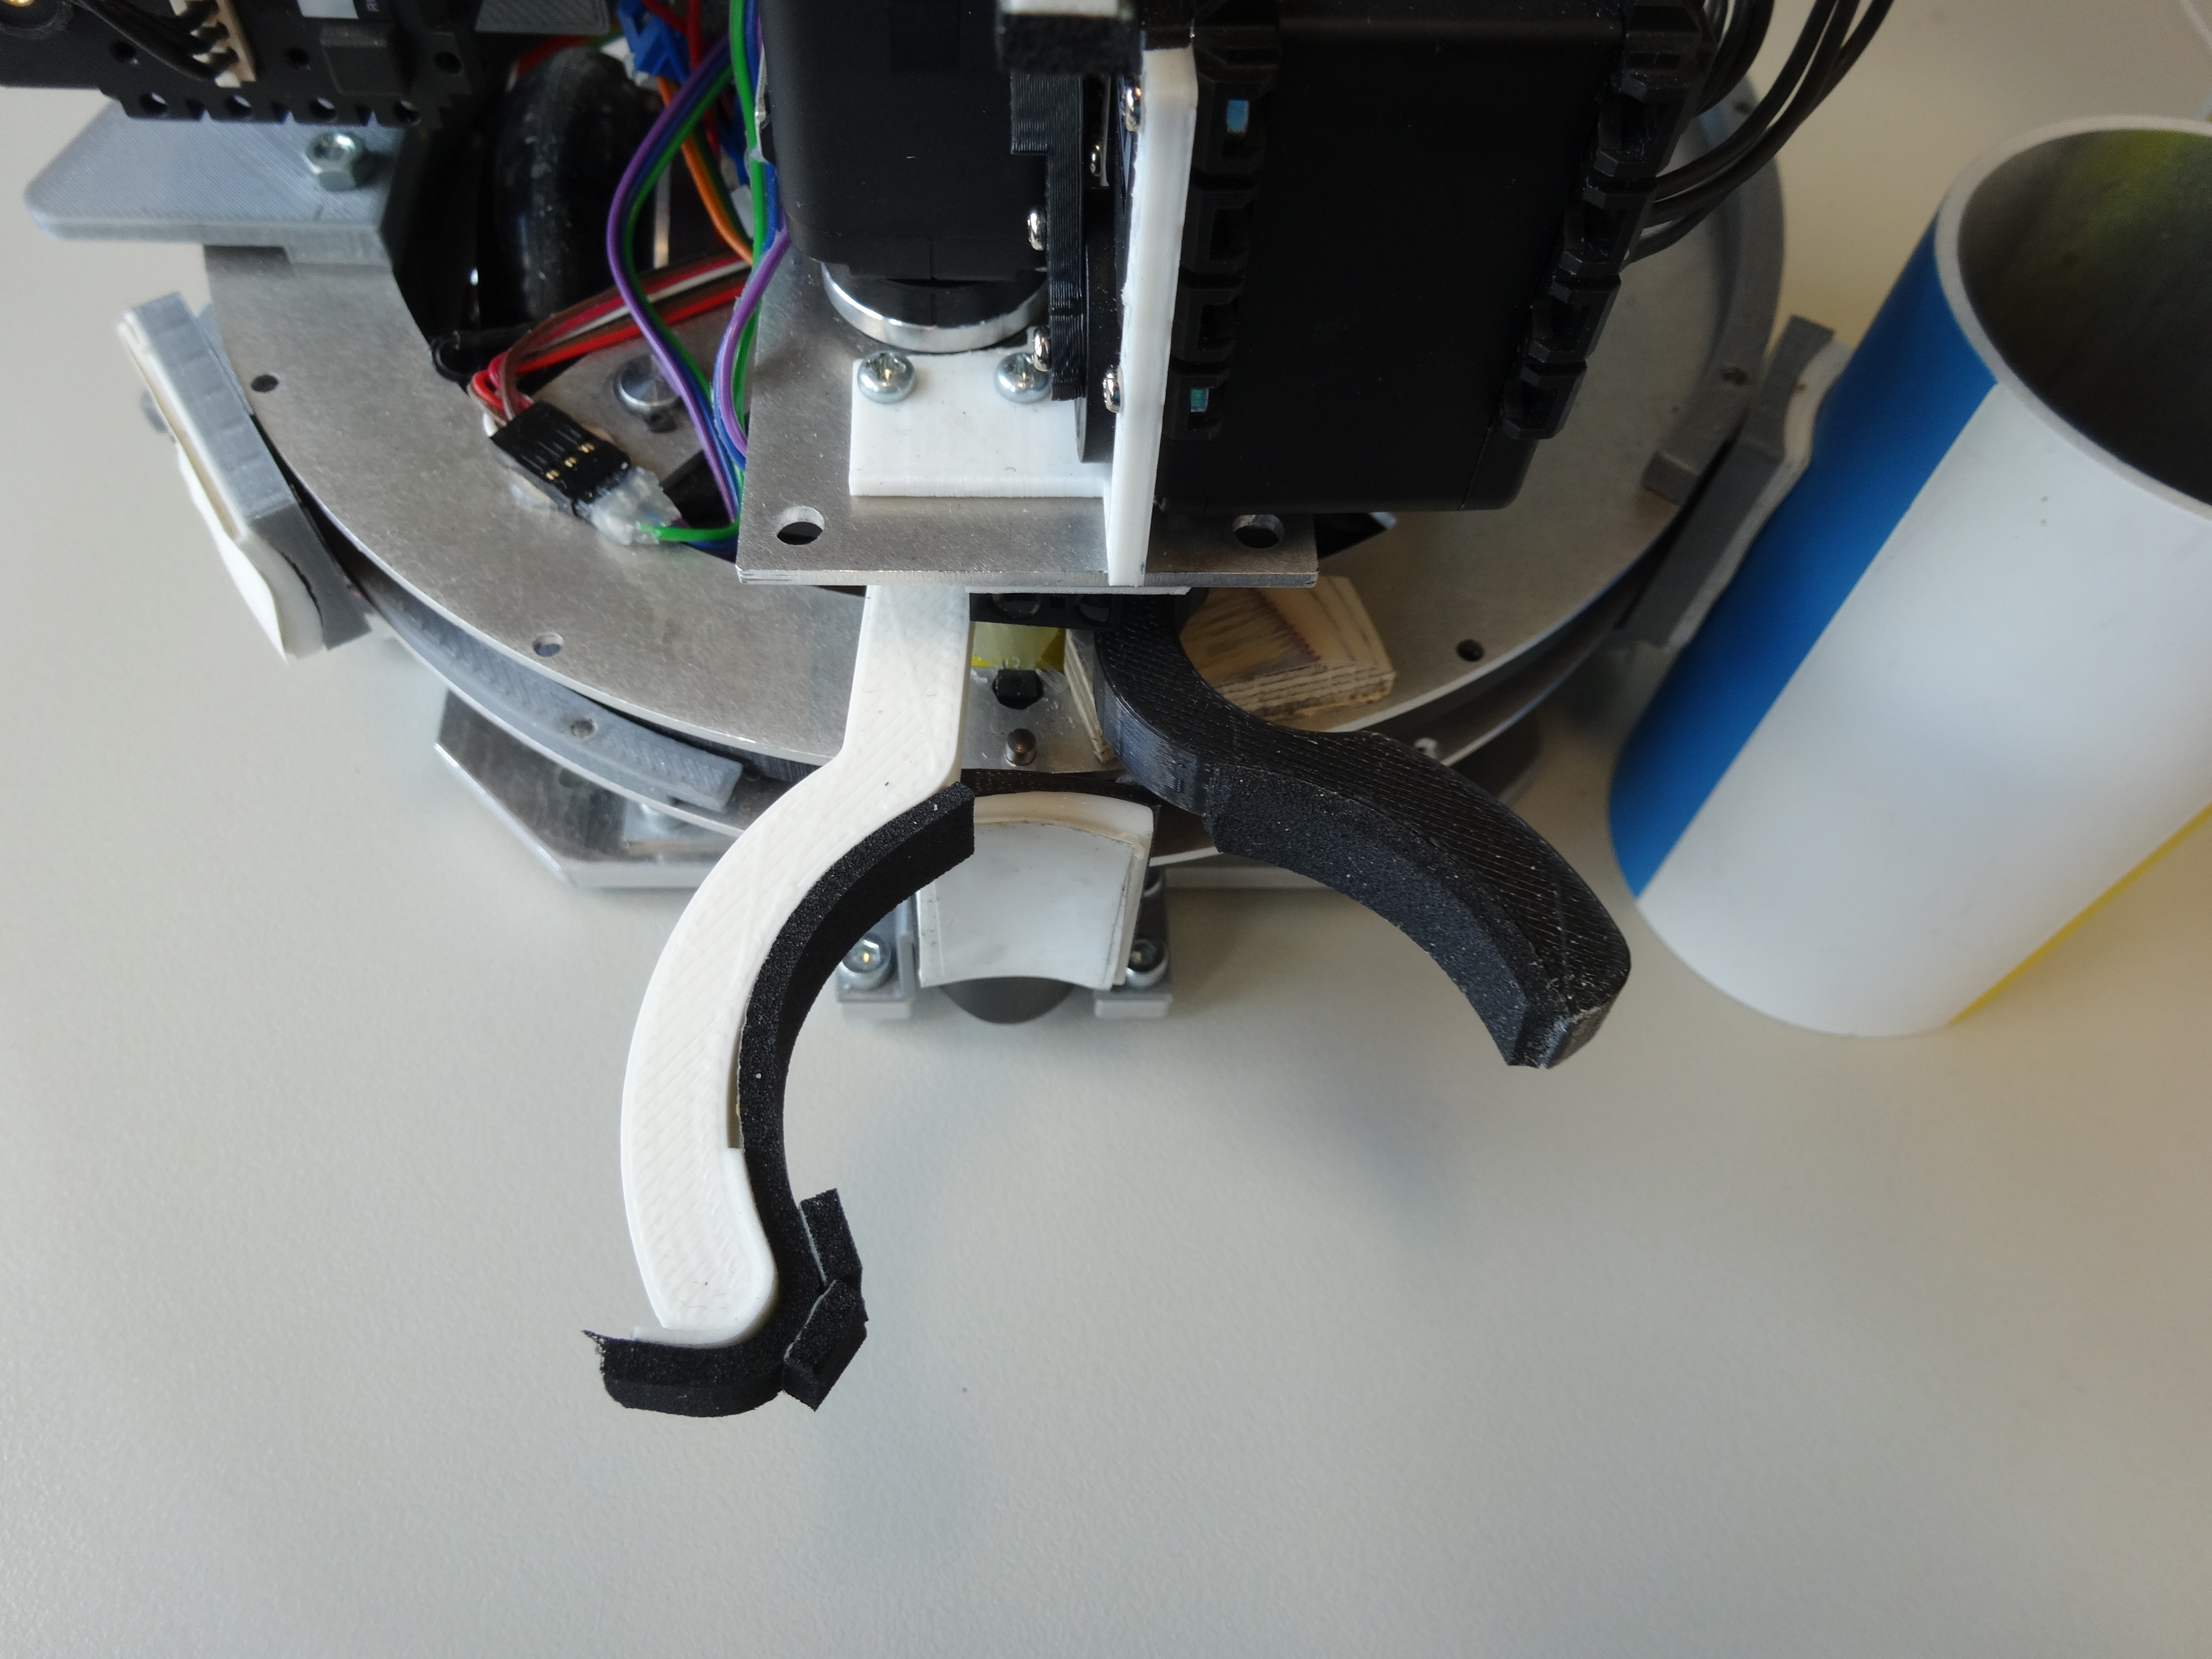
\includegraphics[width = 0.6\columnwidth] {../images/presentation/kleinerRoboter/Greifer.JPG}\\\vspace{1em}
			\includegraphics[width = 0.5\columnwidth, angle=90, origin=c]  {../images/presentation/kleinerRoboter/Pressfinger.JPG}\\
			\column{0.5\textwidth}
			\centering
			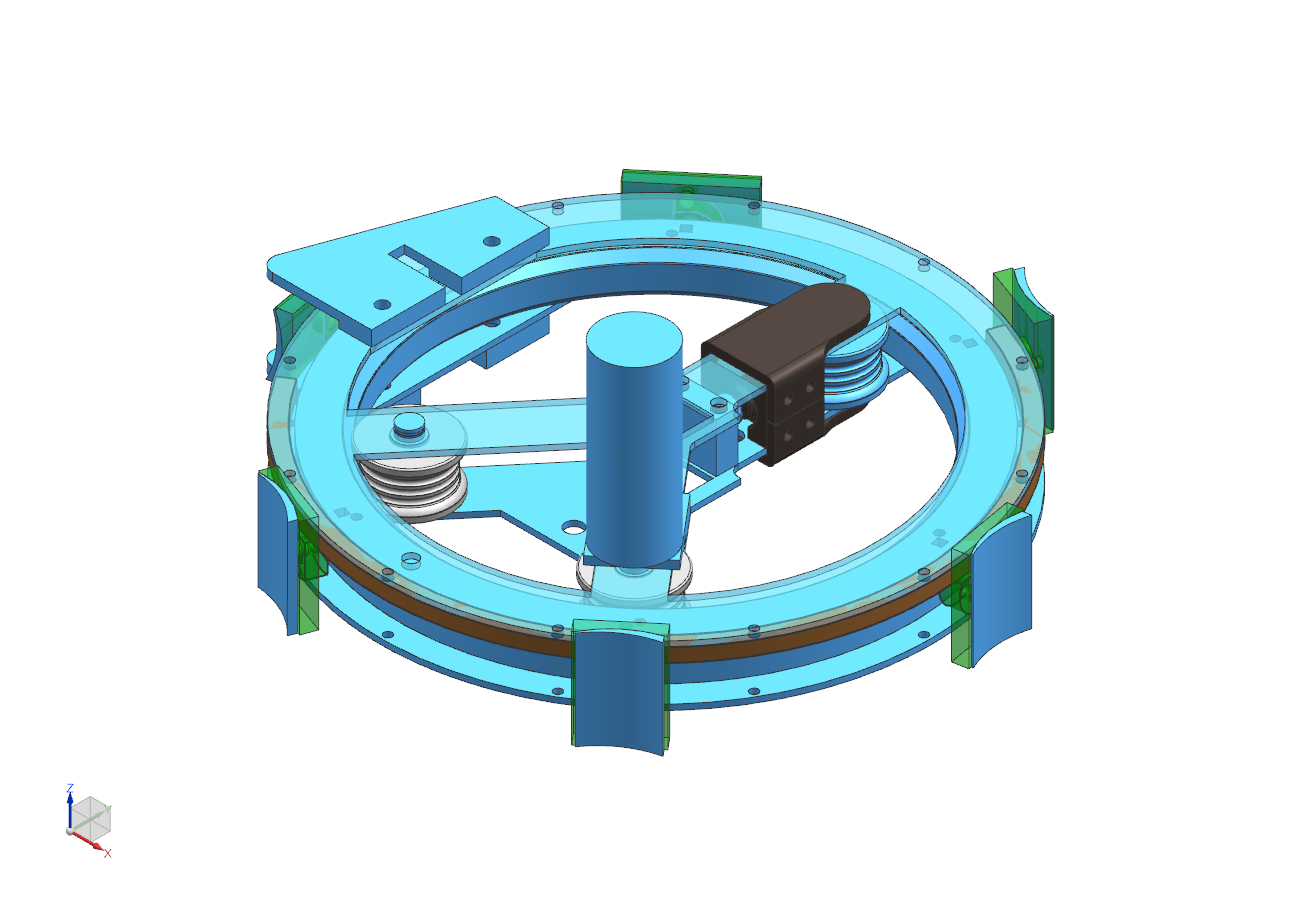
\includegraphics[width = 0.7\columnwidth]{../images/presentation/kleinerRoboter/Ring.png}\\\vspace{1em}
			\includegraphics[width = 0.6\columnwidth]{../images/presentation/kleinerRoboter/Drehen.JPG}\\		
		\end{columns}
	\end{figure}
\end{frame}

%todo viel zu viel!

%\begin{frame}
%	\frametitle{Grosser Roboter}	
%	\framesubtitle{Supportrad}
%	\begin{columns}
%		\begin{column}{0.42 \textwidth}
%			\begin{itemize}
%				\item nicht benötigt
%			\end{itemize}
%		\end{column}
%		\begin{column}{0.58 \textwidth}
%			\vspace{-2.8em}
%			\begin{figure}[h]
%				\centering
%				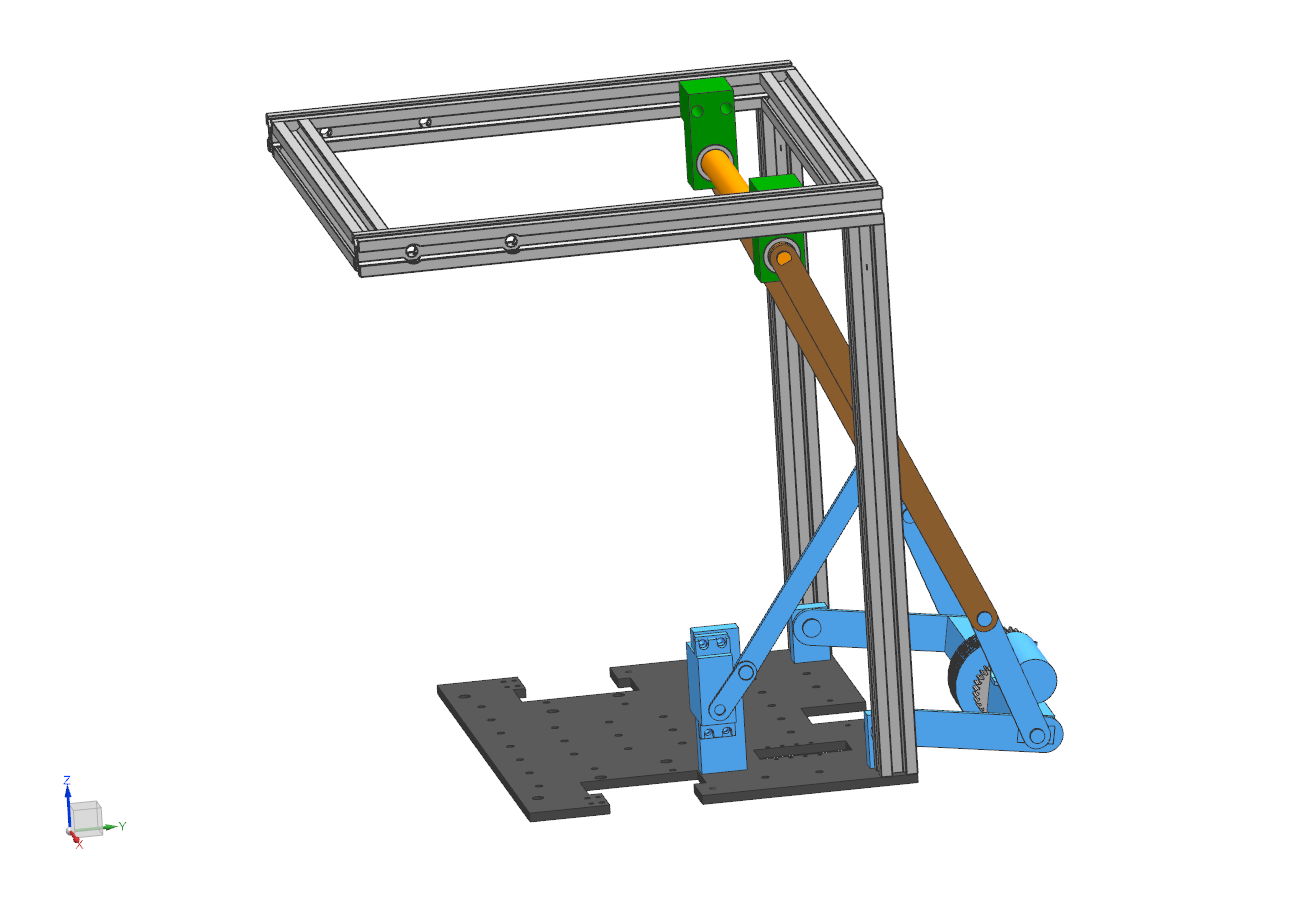
\includegraphics[width = 1 \textwidth]{../images/presentation/supportrad.png}
%			\end{figure}
%		\end{column}
%	\end{columns}
%\end{frame}
%
%\begin{frame}
%	\frametitle{Grosser Roboter}
%	\framesubtitle{Walze und Leitplanke}
%	\begin{columns}
%		\begin{column}{0.6 \textwidth}
%			\begin{itemize}
%				\item Aufnahme der \textit{Titanium Ores}
%				\item Spielelemente dürfen nicht beschäditgt werden
%				\item Gummibänder und Kabelbinder
%				\item Bereichsvergrösserung durch Leitplanken
%			\end{itemize}
%		\end{column}
%		\begin{column}{0.4 \textwidth}
%			\vspace{-2.5em}
%			\begin{figure}[h]
%				\centering
%				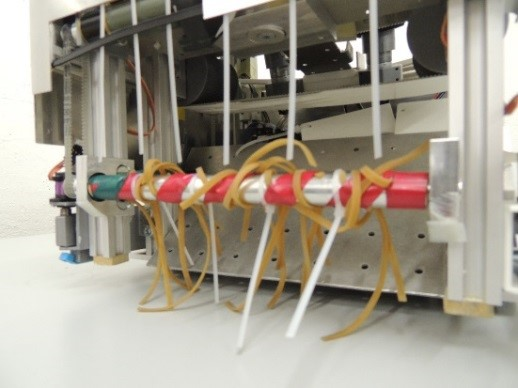
\includegraphics[width = 0.9 \textwidth]{../images/presentation/walze.jpg}
%			\end{figure}
%			\vspace{-2.2em}
%			\begin{figure}[h]
%				\centering
%				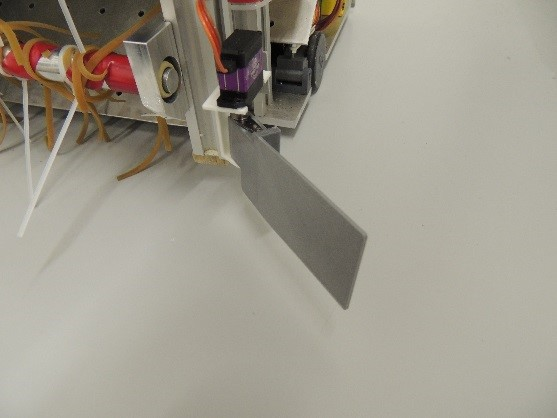
\includegraphics[width = 0.9 \textwidth]{../images/presentation/leitplanke.jpg}
%			\end{figure}
%		\end{column}
%	\end{columns}
%\end{frame}
%
%\begin{frame}
%	\frametitle{Grosser Roboter}
%	\framesubtitle{Riemen und Abstreifvorrichtung}
%	\begin{columns}
%	\begin{column}{0.6 \textwidth}
%		\begin{itemize}
%			\item Beförderung zum Schussmechanismus
%			\item Klebeband
%			\item mechanischer Abstreifer
%			\item \textit{Titanium Ores} von \textit{Moon Rocks} trennen
%		\end{itemize}
%	\end{column}
%	\begin{column}{0.4 \textwidth}
%		\vspace{-2.5em}
%		\begin{figure}[h]
%			\centering
%			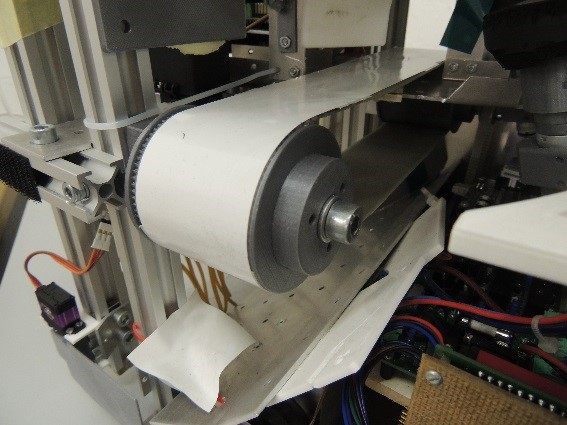
\includegraphics[width = 0.9 \textwidth]{../images/presentation/riemen.jpg}
%		\end{figure}
%		\vspace{-2.2em}
%		\begin{figure}[h]
%			\centering
%			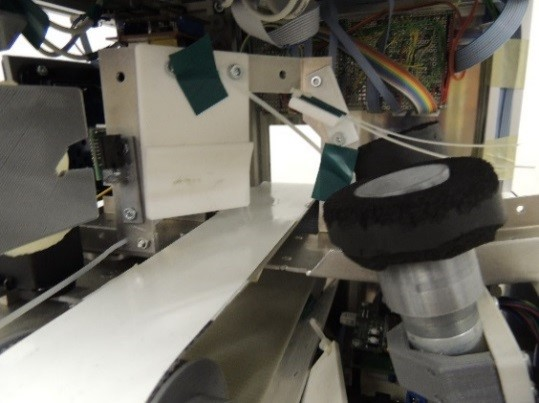
\includegraphics[width = 0.9 \textwidth]{../images/presentation/abstreifvorrichtung.jpg}
%		\end{figure}
%	\end{column}
%\end{columns}
%\end{frame}
%
%\begin{frame}
%	\frametitle{Grosser Roboter}
%	\framesubtitle{Schussmechanismus}
%		\begin{columns}
%		\begin{column}{0.42 \textwidth}
%			\begin{itemize}
%				\item schiesst \textit{Titanium Ores} in die \textit{Cargo Bay}
%				\item zwei sich drehende Rollen
%				\item variable Distanz und Richtung
%				\item Berechnung anhand der Position
%			\end{itemize}
%		\end{column}
%		\begin{column}{0.58 \textwidth}
%			\vspace{-2.8em}
%			\begin{figure}[h]
%				\centering
%				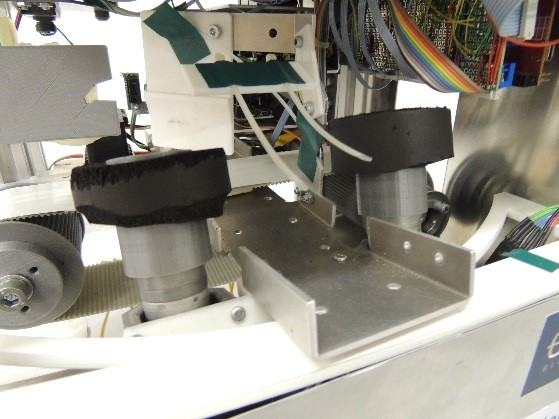
\includegraphics[width = 1 \textwidth]{../images/presentation/schussmechanismus.jpg}
%			\end{figure}
%		\end{column}
%	\end{columns}
%\end{frame}
%
%\subsection{Kleiner Roboter}
%
%\begin{frame}
%	\frametitle{Kleiner Roboter}
%	\framesubtitle{Modulaufnahme}
%	Mithilfe eines Scherenzugs sollten die \textit{Lunar Modules} aus den Raketen gezogen werden.
%	Dieses Konzept funktionierte nicht wunschgemäss und wurde deshalb durch einen Greifer und einen Pressfinger ersetzt.\\
%	
%	\begin{figure}
%		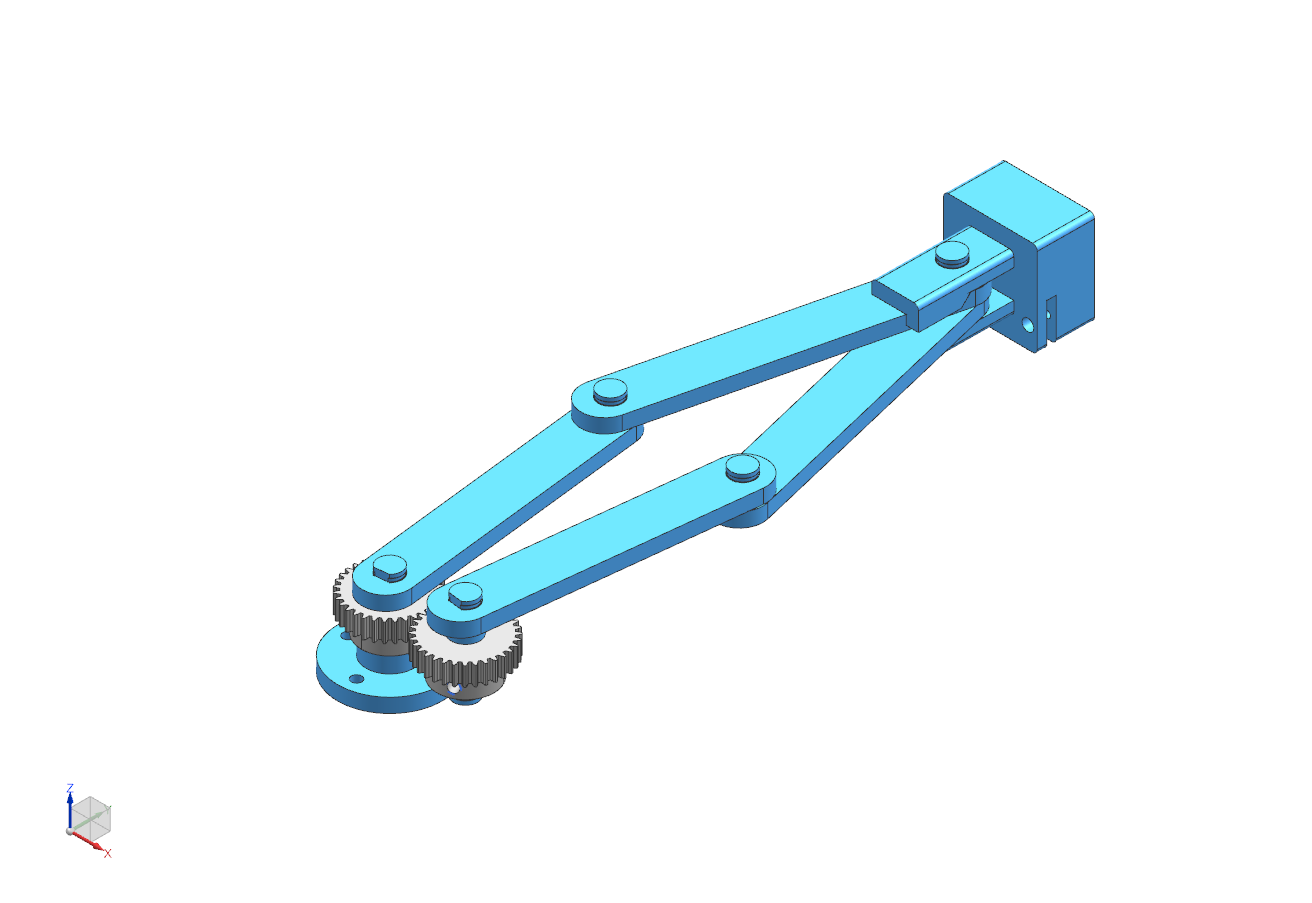
\includegraphics[height = 3 cm]{../images/presentation/kleinerRoboter/Schere.png}
%		\hspace{1em}
%		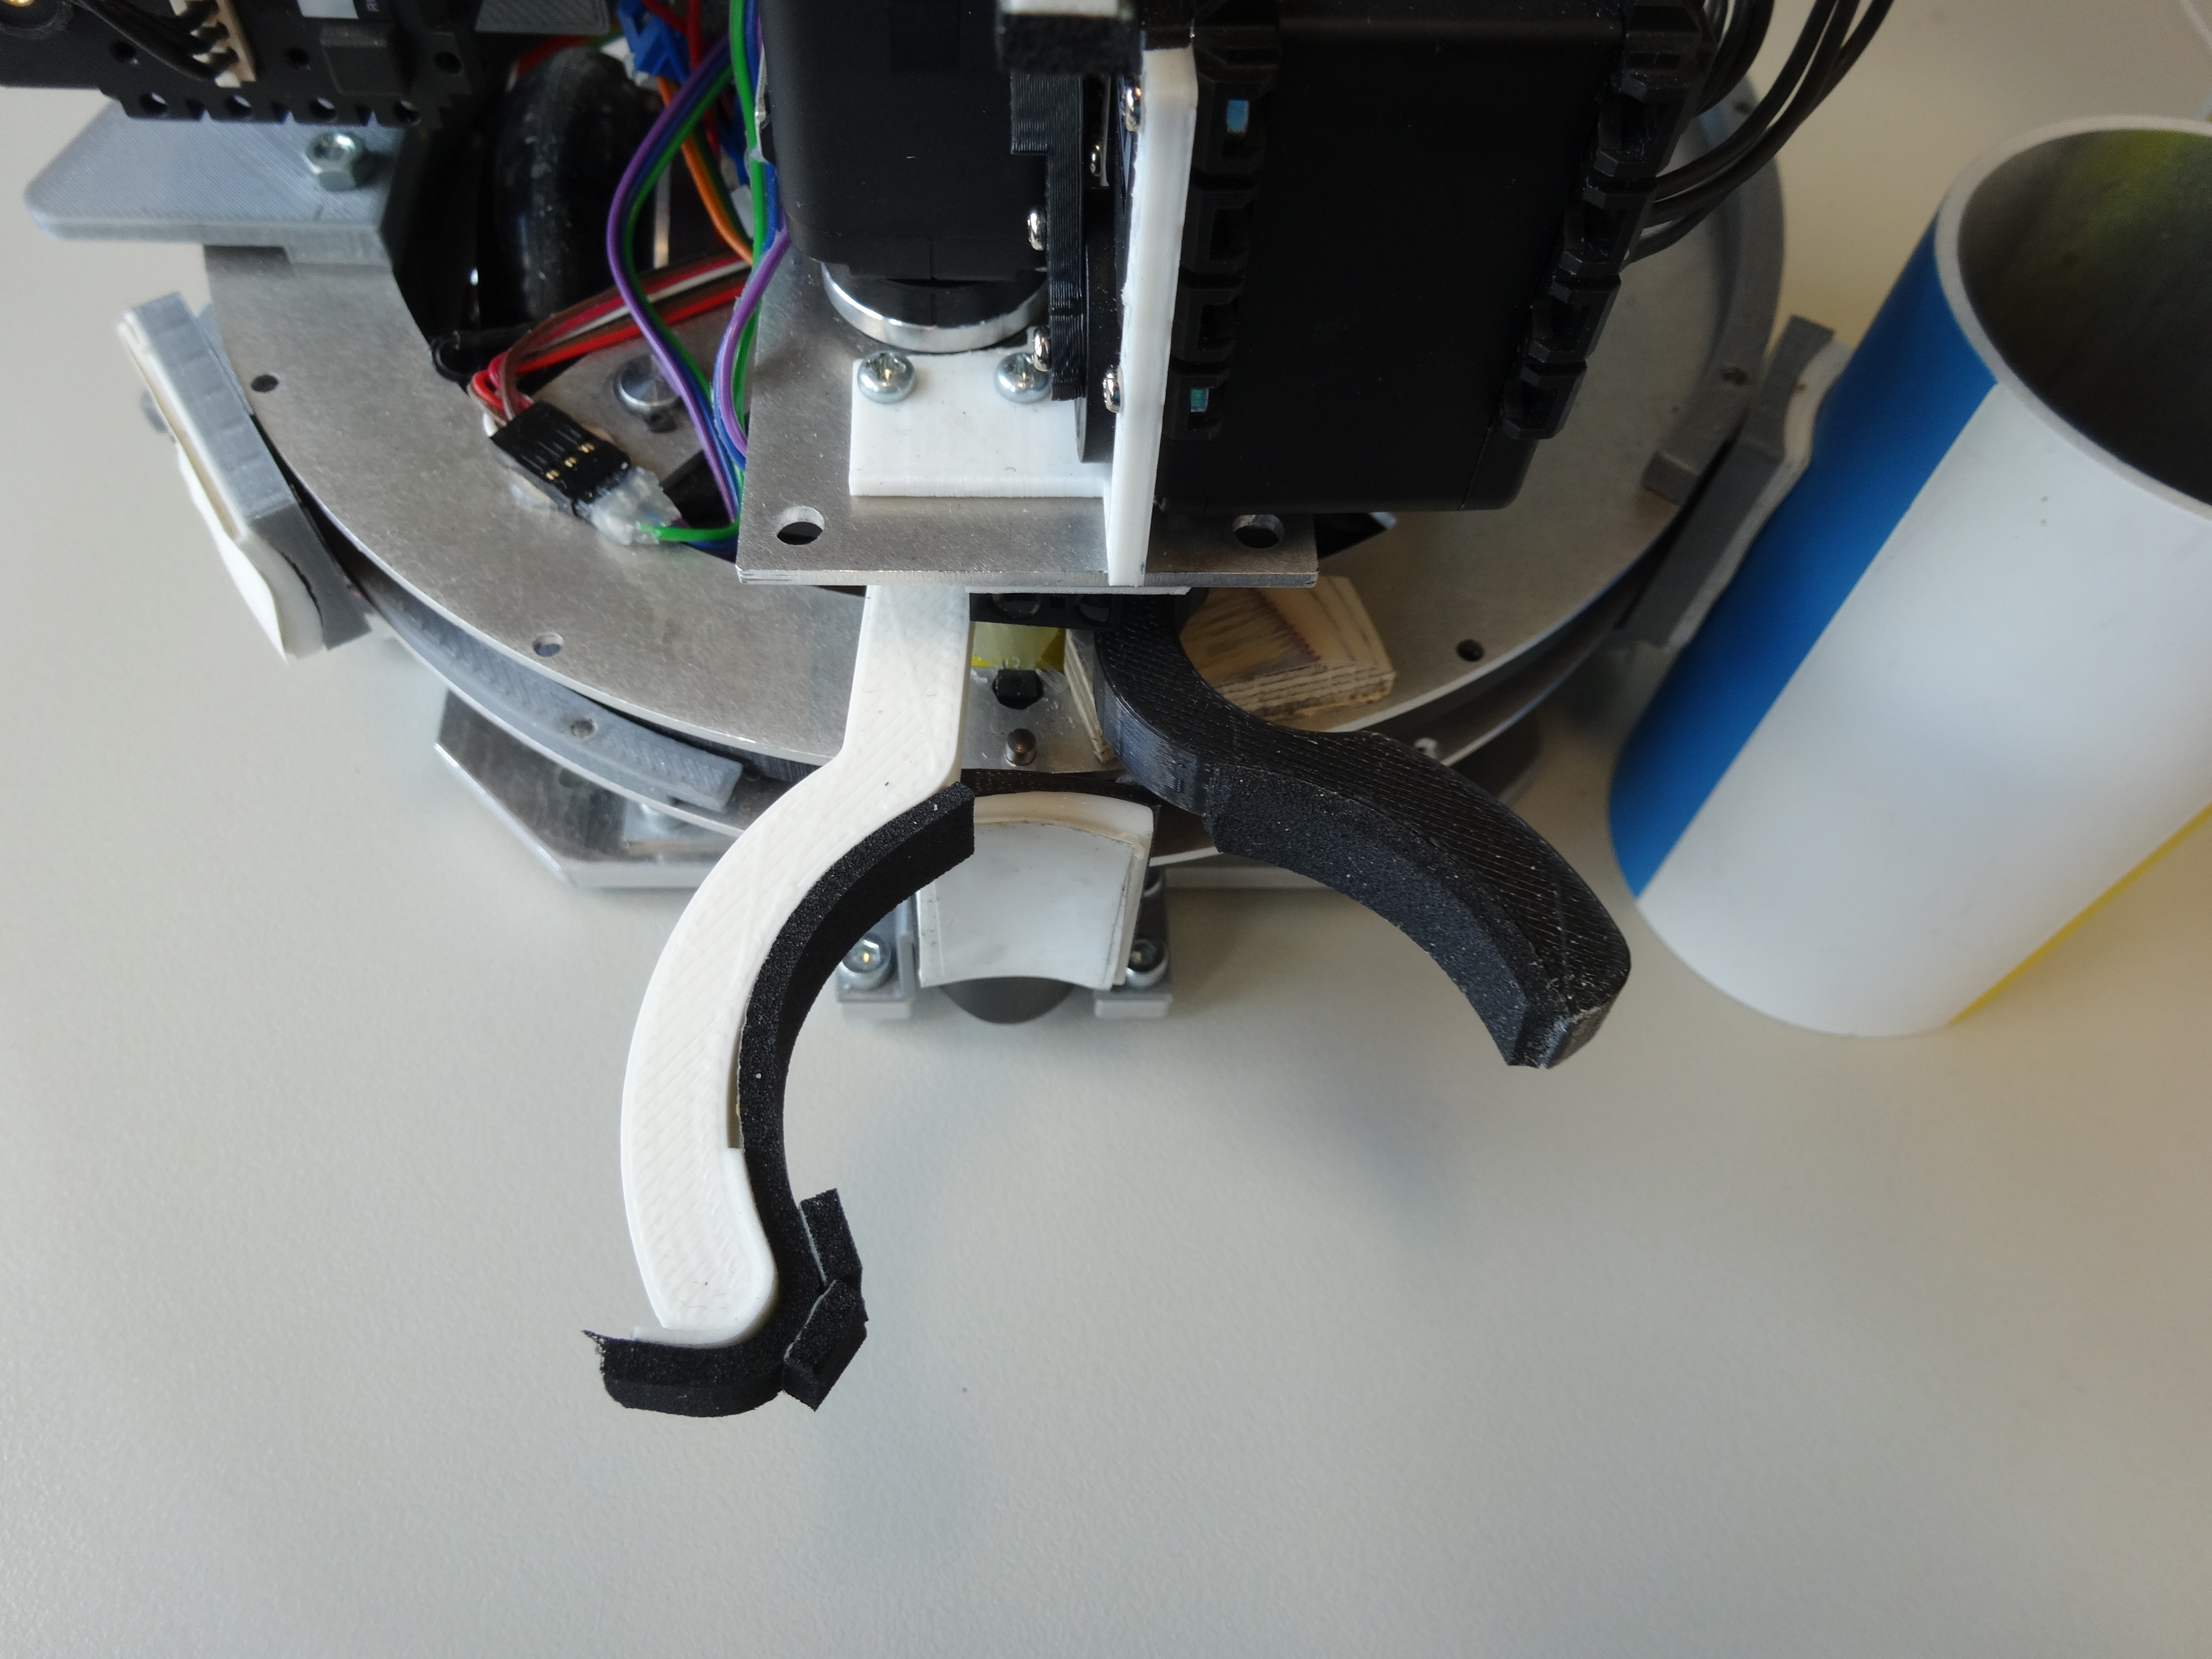
\includegraphics[height = 3 cm]{../images/presentation/kleinerRoboter/Greifer.JPG}
%		\hspace{2em}
%		\includegraphics[angle = 90, height = 3 cm]{../images/presentation/kleinerRoboter/Pressfinger.JPG}
%	\end{figure}
%\end{frame}
%
%\begin{frame}
%	\frametitle{Kleiner Roboter}
%	\framesubtitle{Ring}
%	Die \textit{Lunar Modules} haften während dem Transport an den Klebestellen des Rings.
%	Durch drehen des Rings werden sie gekippt und abgestreift.
%	\begin{figure}
%		\centering
%		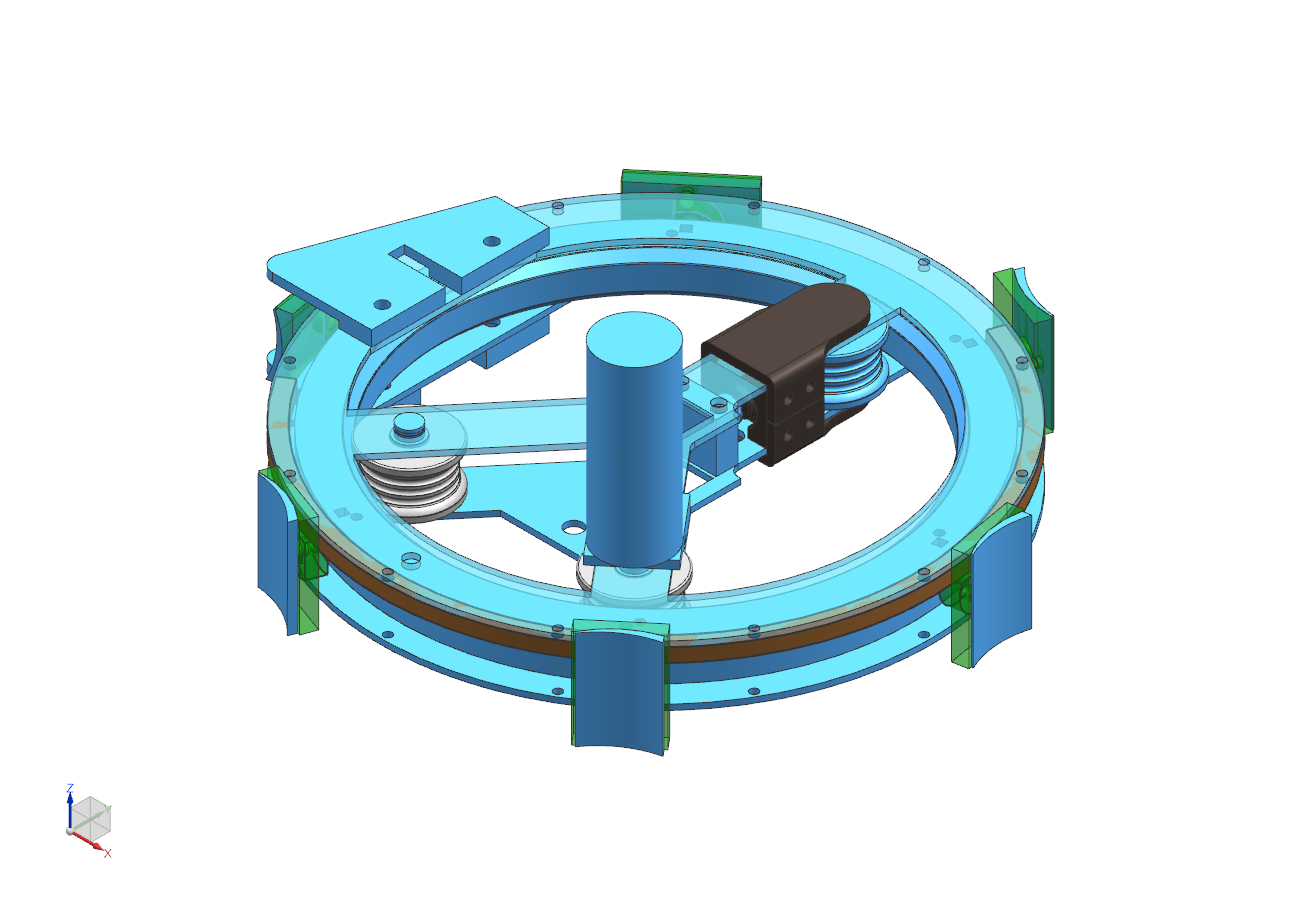
\includegraphics[height = 4 cm]{../images/presentation/kleinerRoboter/Ring.png}
%	\end{figure}
%\end{frame}
%
%\begin{frame}
%	\frametitle{Kleiner Roboter}
%	\framesubtitle{Drehmechanismus}
%	Ein Arm mit einem Farbsensor und einem Rad kann ausgeklappt werden um \textit{Lunar Modules} zu drehen oder zu verschieben.
%	\begin{figure}
%		\centering
%		\includegraphics[height = 4 cm]{../images/presentation/kleinerRoboter/Drehen.JPG}
%	\end{figure}
%\end{frame}
  
  %Mainboard und Strategie-Einheit
  \section{Strategie-Einheit}

\begin{frame}
	\frametitle{Übersicht}
	
	\begin{itemize}
		\item Verantwortlich für alle Aktionen während dem Spiel
		\item Dynamische Jobauswahl
		\item Pfadsuche
		\item Ausweichmanöver bei Kollisionswarnung
		\item Kommunikation mit Partner
	\end{itemize}
	
\end{frame}

\begin{frame}
	\frametitle{Aufgaben (\textit{Jobs})}
	
	\begin{figure}
		\begin{tikzpicture} [scale=0.6, transform shape]
			\coordinate (strategySize) at (18.5,10);
			\def\top{9.4};
			\def\sep{0.3};
			\def\varHeight{0.8};
			\def\varWidth{4};
			\def\jobHeight{8.5};
			\def\jobWidth{13.3};
			\def\jobTop{8.3};
			\def\fsmHeight{\jobTop+3*\sep};
			\def\fsmWidth{\jobWidth-4*\sep-\varWidth};
			\def\fsmText{4.05};
			
			\coordinate (jobStart) at (\sep+\varWidth+\sep, \top-\sep);
			\draw (0,0) rectangle (strategySize) node[pos=0.5, shift={(0, 4.5)}]{\Large \textbf{strategy}}; %strategy box
			
			%strategy components
			\draw (\sep, \top-\sep-0*\sep-0*\varHeight) rectangle ++(\varWidth, -\varHeight) node[pos=0.5]{Status variables};
			\draw (\sep, \top-\sep-1*\sep-1*\varHeight) rectangle ++(\varWidth, -\varHeight) node[pos=0.5]{current Job};
			\draw (\sep, \top-\sep-1*\sep-2*\varHeight) [draw=none] rectangle ++(\varWidth, -\varHeight) node[pos=0.5]{$\vdots$};
			
			%jobs
			\draw (jobStart) [shift={(1*\sep, -1*\sep)}, fill=gray!10, visible on=<2->] rectangle ++(\jobWidth, -\jobHeight);
			\draw (jobStart) [shift={(0.5*\sep, -0.5*\sep)}, fill=gray!10, visible on=<2->] rectangle ++(\jobWidth, -\jobHeight);
			\draw (jobStart) [shift={(0*\sep, -0*\sep)}, fill=gray!10, visible on=<2->] rectangle ++(\jobWidth, -\jobHeight) node[pos=0.5, shift={(0, 0.45*\jobHeight)}] {\textbf{Job}};
			
			%job content
			\begin{scope} [shift={(\sep+\varWidth+\sep+\sep, \jobTop)}]
				\draw (0,-0*\varHeight-0*\sep) [fill=white, visible on=<3->] rectangle ++(\varWidth, -\varHeight) node[pos=0.5] {ID};
				
				\draw (0,-1*\varHeight-1*\sep) [fill=white, visible on=<3->] rectangle ++(\varWidth, -\varHeight) node[pos=0.5] {currentState};
				
				\draw (1*\sep,-2*\varHeight-3*\sep) [fill=white, visible on=<4->] rectangle ++(\varWidth, -\varHeight);
				\draw (0.5*\sep,-2*\varHeight-2.5*\sep) [fill=white, visible on=<4->] rectangle ++(\varWidth, -\varHeight);
				\draw (0,-2*\varHeight-2*\sep) [fill=white, visible on=<4->] rectangle ++(\varWidth, -\varHeight) node[pos=0.5] {requirementFunction()};
				
				\draw (1*\sep,-3*\varHeight-5*\sep) [fill=white, visible on=<4->] rectangle ++(\varWidth, -\varHeight);
				\draw (0.5*\sep,-3*\varHeight-4.5*\sep) [fill=white, visible on=<4->] rectangle ++(\varWidth, -\varHeight);
				\draw (0,-3*\varHeight-4*\sep) [fill=white, visible on=<4->] rectangle ++(\varWidth, -\varHeight) node[pos=0.5] {priorityFunction()};
				
				\draw (0,-4*\varHeight-6*\sep) [fill=white, visible on=<6->] rectangle ++(\varWidth, -\varHeight) node[pos=0.5] {Target};
				
				\draw (0,-5*\varHeight-6*\sep) [draw=none, visible on=<6->] rectangle ++(\varWidth, -\varHeight) node[pos=0.5]{$\vdots$};
				
				\begin{scope} [shift={(\varWidth+2*\sep, 0)}]
				
					\draw (0,0) [fill=white, visible on=<5->] rectangle ++(\fsmWidth, -\fsmHeight);
					\node [shift={(\fsmText, -0.4)}, visible on=<5->] {State Machine};
					\node [shift={(\fsmText, -0.8)}, anchor=north, visible on=<5->] {
						\footnotesize
						\begin{tabular}{|c|c|c|c|}
							\hline
							currentState & evaluation() & task() & nextState \\ \hline \hline
							& & & \\ \hline
							& & & \\ \hline
							& & & \\ \hline
							& & & \\ \hline
							& & & \\ \hline
							& & & \\ \hline
							& & & \\ \hline
							& & & \\ \hline
							& & & \\ \hline
							& & & \\ \hline
							& & & \\ \hline
							& & & \\ \hline
							& & & \\ \hline
							& & & \\ \hline
						\end{tabular}
					};
				
				\end{scope}
			
			\end{scope}
		
		\end{tikzpicture}
	\end{figure}
\end{frame}

\begin{frame}
	\frametitle{Pfadsuche und Spielfeld}
	\vspace{-1.5em}
	\only<1>{\begin{figure}\includegraphics[scale=0.035]{../images/spielfeld/playingAreaPlain.pdf}\end{figure}}	\only<2>{\begin{figure}\includegraphics[scale=0.035]{../images/spielfeld/playingAreaAreas.pdf}\end{figure}}	\only<3>{\begin{figure}\includegraphics[scale=0.035]{../images/spielfeld/playingAreaWaypoint.pdf}\end{figure}}	\only<4>{\begin{figure}\includegraphics[scale=0.035]{../images/spielfeld/playingAreaGraph.pdf}\end{figure}}
	\only<5>{\begin{figure}\includegraphics[scale=0.035]{../images/spielfeld/playingAreaPath1.pdf}\end{figure}}
	\only<6>{\begin{figure}\includegraphics[scale=0.035]{../images/spielfeld/playingAreaPath2.pdf}\end{figure}}
	\only<7>{\begin{figure}\includegraphics[scale=0.035]{../images/spielfeld/playingAreaPath3.pdf}\end{figure}}
	
\end{frame}

\begin{frame}
	\frametitle{\textit{collision handling}}
	\vspace{-1.5em}
	\only<1>{\begin{figure}\includegraphics[scale=0.035]{../images/spielfeld/playingAreaPath4.pdf}\end{figure}}
	\only<2>{\begin{figure}\includegraphics[scale=0.035]{../images/spielfeld/playingAreaPath5.pdf}\end{figure}}
	\only<3>{\begin{figure}\includegraphics[scale=0.035]{../images/spielfeld/playingAreaPath6.pdf}\end{figure}}
\end{frame}

\begin{frame}
	\frametitle{Erkentnisse und Ergebnis}
	
	\begin{itemize}
		\item Wiederverwendbarkeit der Jobs
		\item Komplexität
		\item Ausweichpfade nur sehr selten möglich
	\end{itemize}
	
\end{frame}
  
  %Fahrkontroller
  \section{Fahrcontroller}

\begin{frame}
	\frametitle{Anpassungen}	
	\begin{columns}
		\begin{column}{0.6 \textwidth}
			\begin{itemize}
				\item Studienarbeit als Basis
				\item Interface auf Mainboard
				\item Kommunikation
				\item Rest bei Gleitkommaoperationen
				\item Kalibrierung
			\end{itemize}
		\end{column}
		\begin{column}{0.4 \textwidth}
			\vspace{-2.8em}
			\begin{figure}[h]
				\centering
				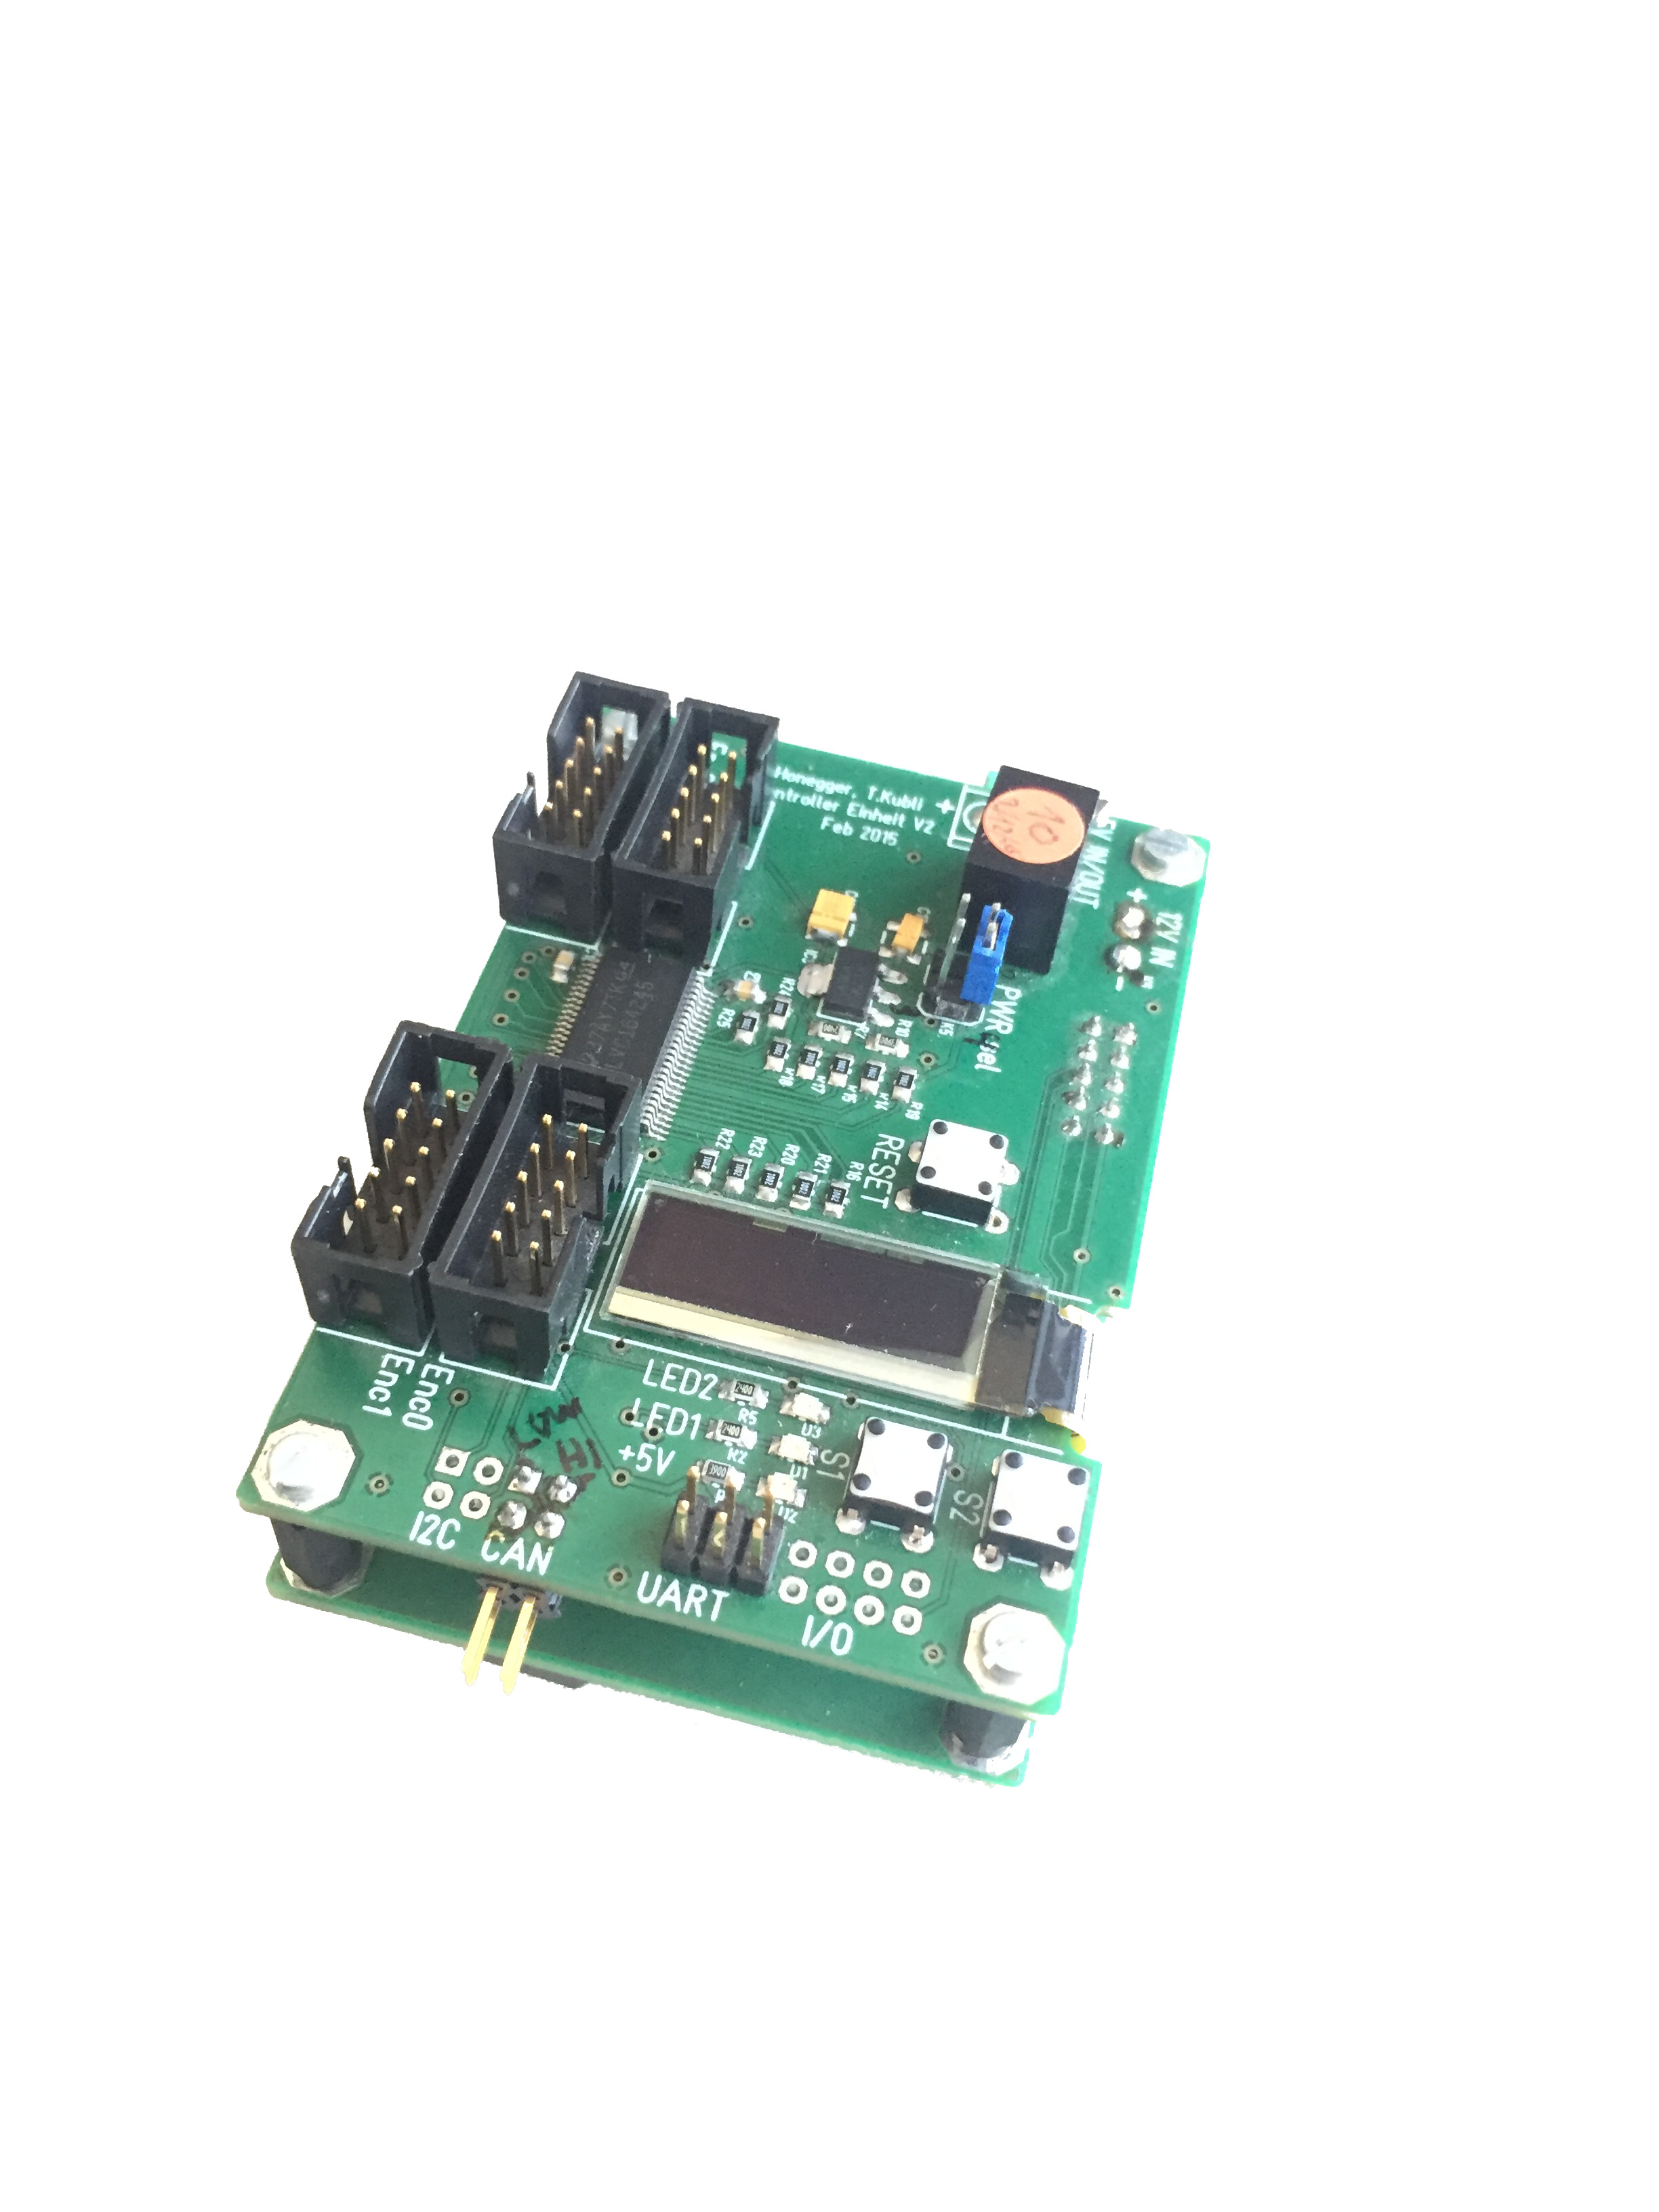
\includegraphics[width = 1 \textwidth]{../images/presentation/dc.jpg}
			\end{figure}
		\end{column}
	\end{columns}
	

\end{frame}

\begin{frame}
	\frametitle{Kalibrieren}
	\begin{itemize}
		\item verbesserte Fehlerberechnung
		\item Bedienung über Display
		\item Konfigurationsdaten auf USB-Stick
		\item getrennte Kalibrierung für Vorwärts- und Rückwärtsfahrt
	\end{itemize}
\end{frame}

\begin{frame}
	\frametitle{Probleme}
	\begin{itemize}
		\item Synchronisation schwierig
		\item kein vorausschauendes Fahren
		\item ungenaues Fahren
		\item Reglereinstellung mühsam
	\end{itemize}
\end{frame}
  
  %Gegnererkennung
  \section{Gegnererkennung}
\begin{frame}
\frametitle{Gegnererkennung}
\framesubtitle{Komponenten}

\begin{figure}
	\begin{tikzpicture}[scale=1, transform shape]
	\def\height{4cm}
	\node[anchor=south west,inner sep=0] (image) at (0,0) {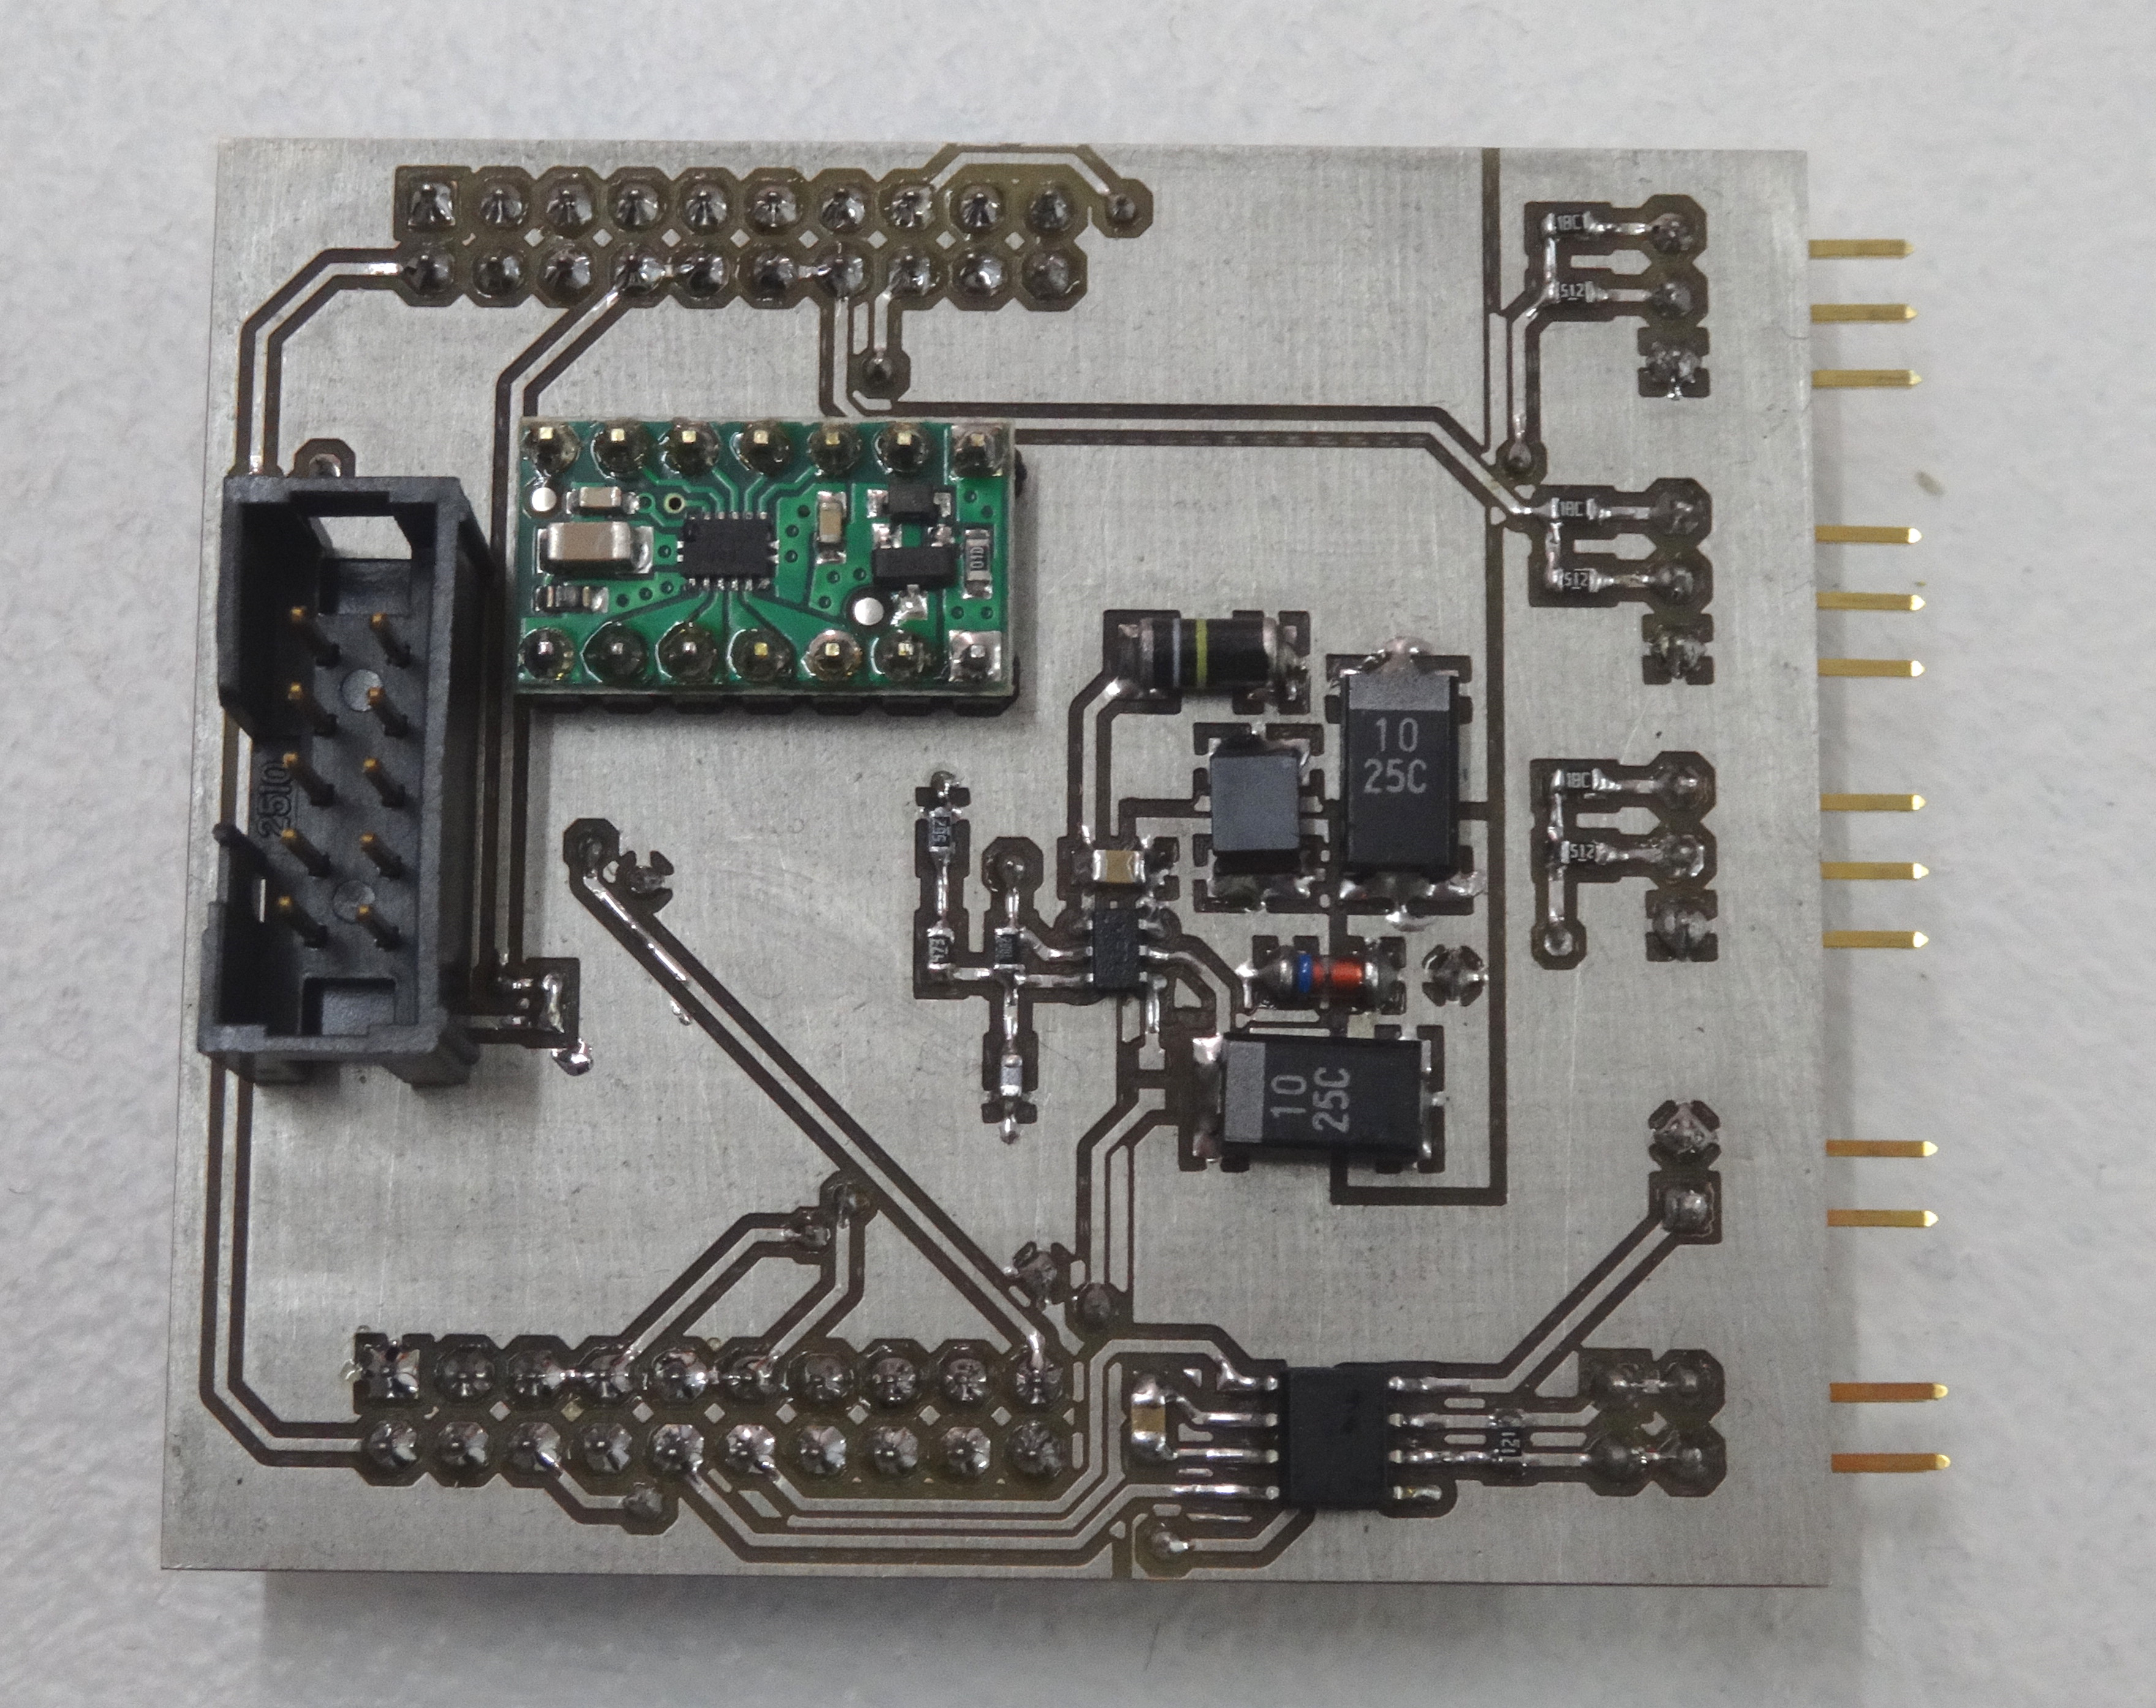
\includegraphics[height=\height] {../images/OD/Adapterboard4.JPG}};
	\begin{scope}[x={(image.south east)},y={(image.north west)}]
		\draw [line width=0.4mm, ->, cGreen] (0.35,1.1) node[left, color=black]{Treiberstufe} -- (0.35,0.75);  
		
		\draw [line width=0.4mm, ->, cGreen] (0.52,1.1) node[right, color=black]{Spannungsregler} -- (0.52, 0.5);
		\draw [line width=0.4mm, ->, cGreen] (0.62,-0.1) node[right, color=black]{CAN-Treiber} -- (0.62, 0.10);
		
		\draw [line width = 0.6mm, -, cRed] (0.15,0.5) to[out = 270, in = 180] (0.5, -0.2);
		\draw [line width = 0.6mm, -, cRed] (0.5, -0.2) -- (1.0, -0.2); 
		%\draw [line width = 0.6mm, -, cRed] (1.0, -0.2) to[out = 0, in = 270] (1.37, 0.1);
		
	\end{scope}
	
	\begin{scope}[xshift=6cm]
		\node[anchor=south west,inner sep=0] (rimage) at (0,0) {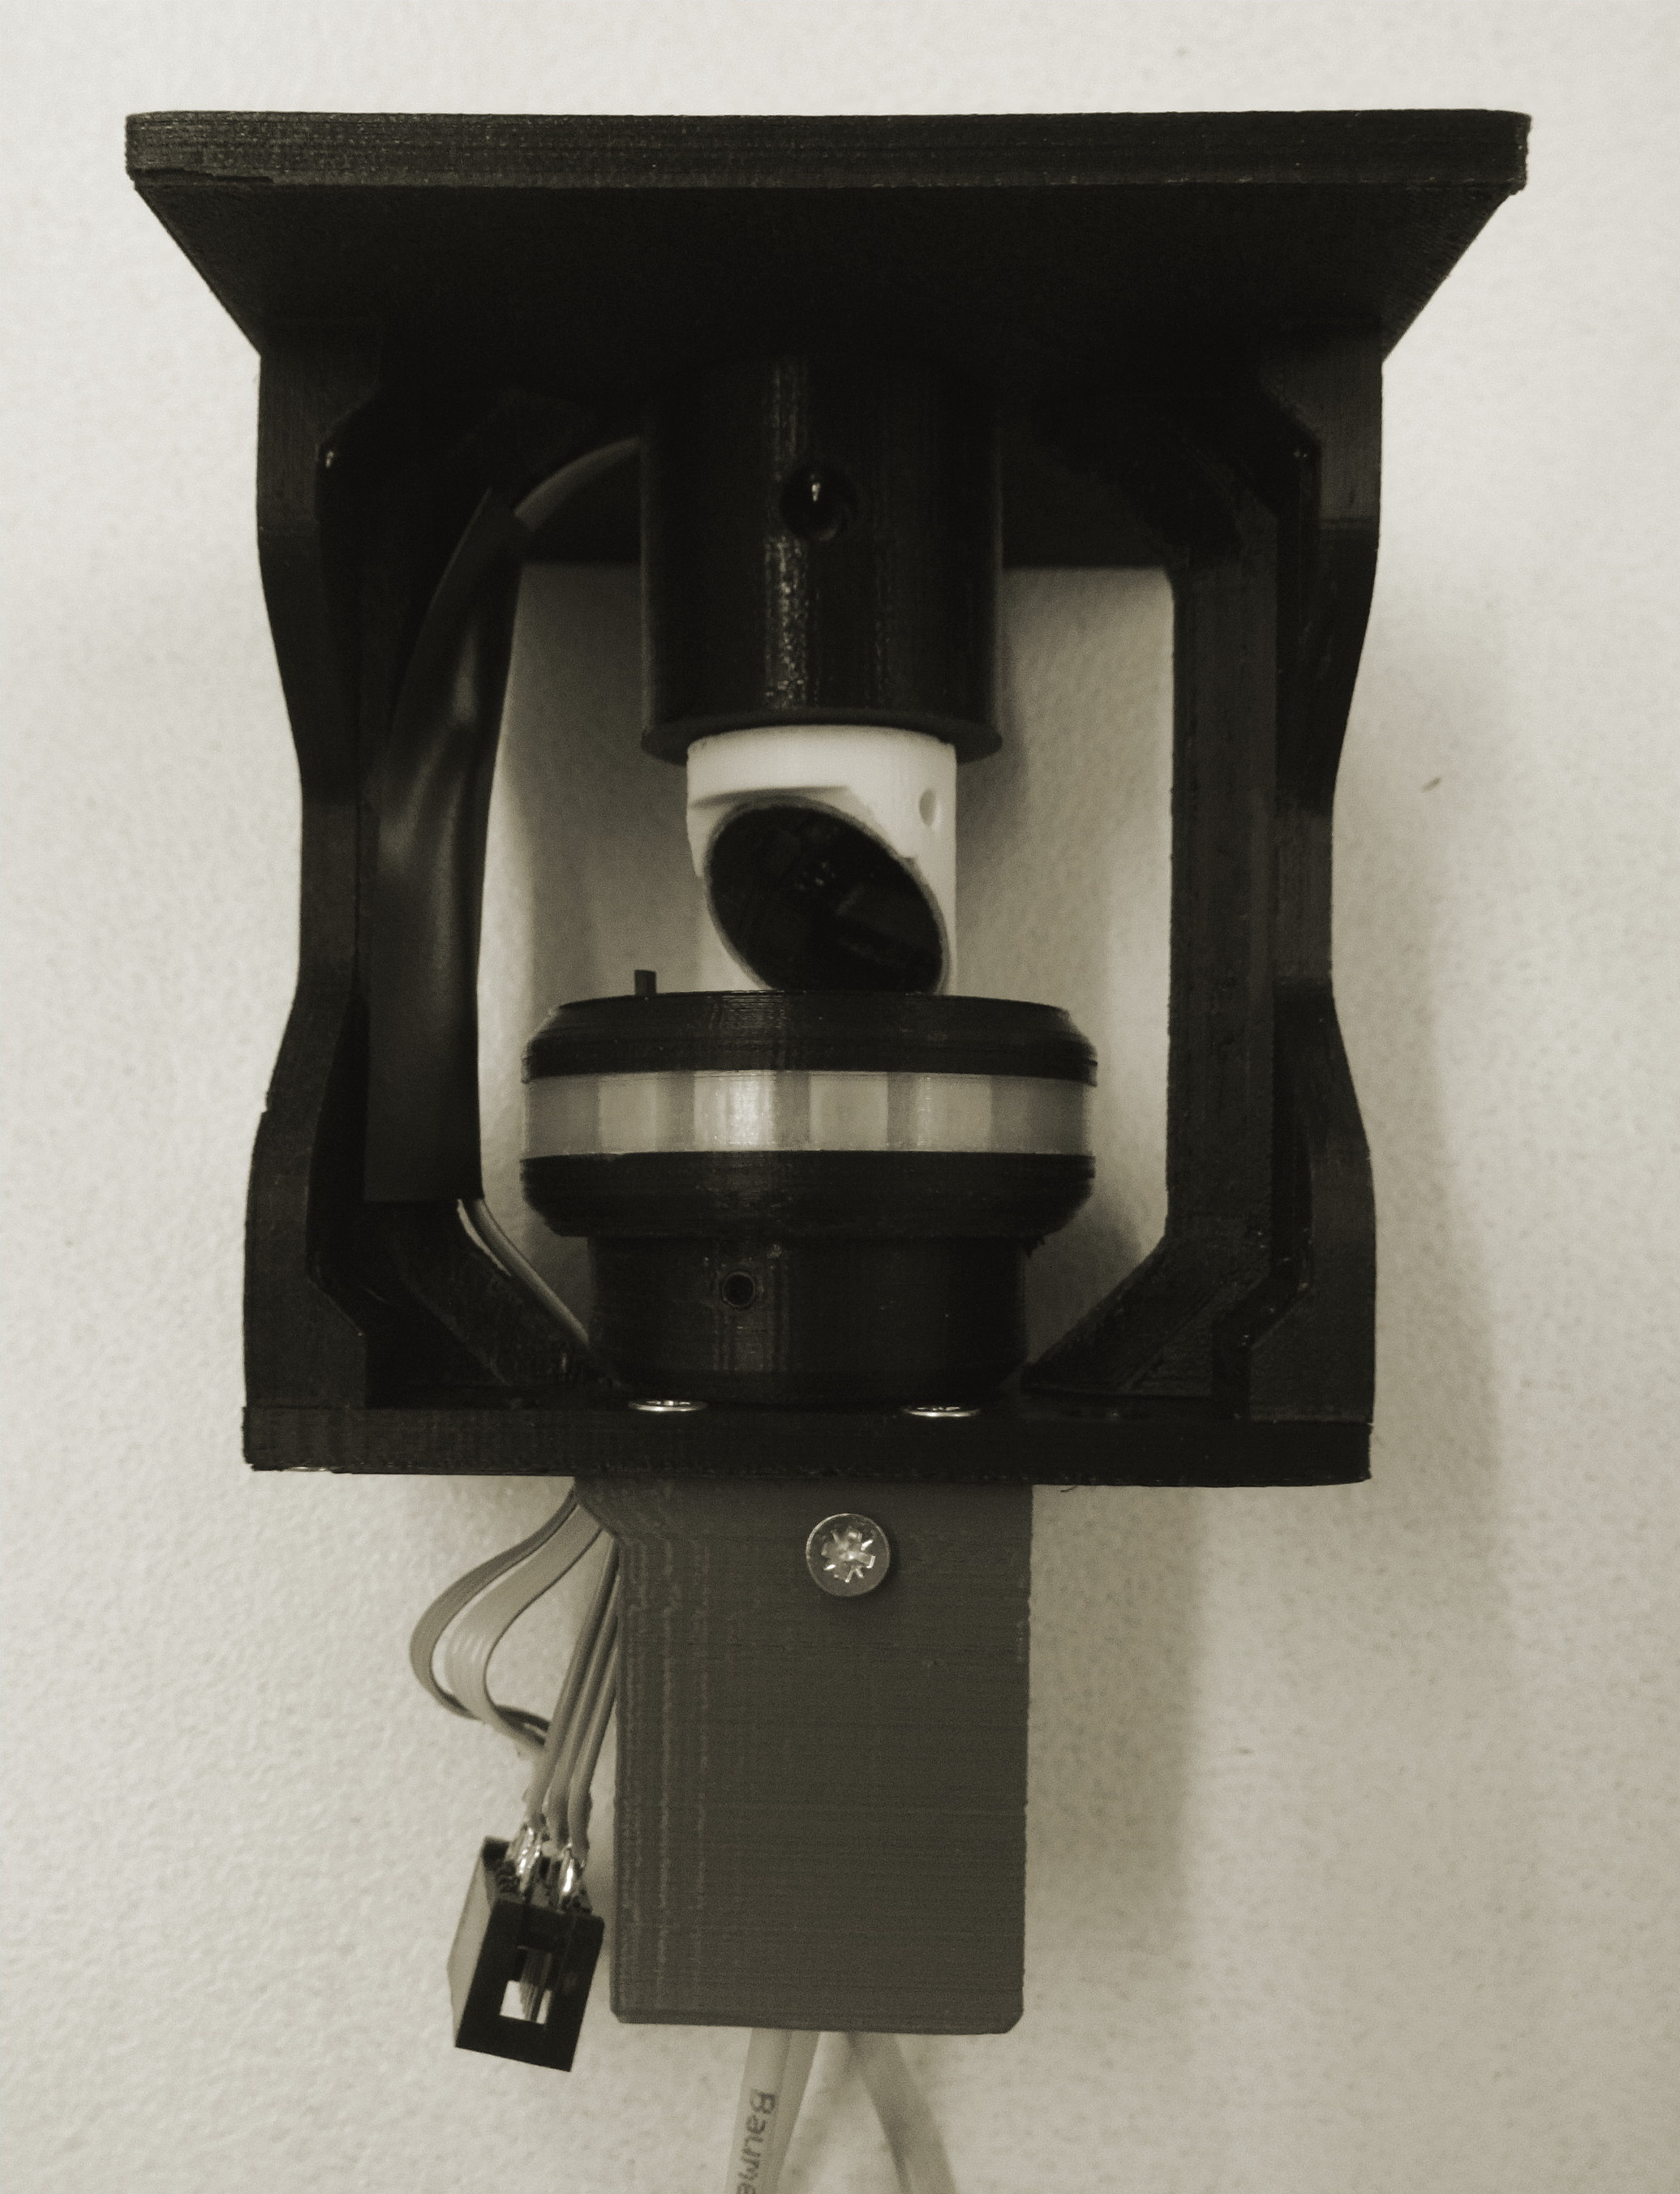
\includegraphics[height=\height] {../images/OD/Kopf3Pres.JPG}};
		\begin{scope}[x={(rimage.south east)},y={(rimage.north west)} ]
		
			\draw [line width=0.4mm, ->, cGreen] (0.5,1.02) node[above, color=black]{Motor und Spiegel} -- (0.5, 0.8);
			\draw [line width=0.4mm, ->, cGreen] (0.55,-0.1) node[right, color=black]{LED-Ring} -- (0.55, 0.4);
			
			\draw [line width = 0.6mm, -, cRed] (-0.32, -0.1985) to[out = 0, in = 270] (0.32, 0.1);
			\draw [line width = 0.4mm, -, cRed] (-0.49, 0.87) -- (-0.49, 0.44);
			\draw [line width = 0.6mm, -, cRed] (-0.49, 0.655) to[out = 0, in = 90] (-0.2, 0.44);
			\draw [line width = 0.6mm, -, cRed] (-0.2, 0.44) -- (-0.2, 0.0);
			\draw [line width = 0.6mm, -, cRed] (-0.2, 0.0) to[out = 270, in = 270] (0.5, 0.0);
		
		\end{scope}
	\end{scope}
	\end{tikzpicture}	
\end{figure}

\end{frame}

\begin{frame}
	\frametitle{Gegnererkennung}
	\framesubtitle{Ausmessung Spiegelhalter}
	
	\begin{figure}
		\centering
		\begin{tikzpicture}[y=-1cm, scale=0.5, transform shape]
		%near right
		\draw [draw=cRed, fill=clRed, fill opacity=0.3] (300:0.6) -- (300:1.95) -- (330:1.65) -- (0:1.6) -- (30:1.8) -- (60:2.4) -- (60:0.8) -- (30:0.65) -- (0:0.5) -- (330:0.5) -- (300:0.6);		
		%middle right
		\draw [draw=cBlue, fill=clBlue, fill opacity=0.3] (300:0.95) -- (330:0.93) -- (0:0.88) -- (30:0.85) -- (60:0.8) -- (60:2.75) -- (30:3.1) -- (0:3.05) -- (330:3.1) -- (300:3.05) -- (300:0.95);
		%middle left
		\draw [draw=cBlue, fill=clBlue, fill opacity=0.3] (120:0.73) -- (150:0.73) -- (180:0.75) -- (210:0.78) -- (240:0.88) -- (240:2.65) -- (210:2.8) -- (180:2.65) -- (150:2.35) -- (120:2.35) -- (120:0.73);
		%far right
		\draw [draw=cGreen, fill=clGreen, fill opacity=0.3] (300:1.25) -- (330:1.25) -- (0:1.1) -- (30:1) -- (60:0.88) -- (60:3.15) -- (30:4.2) -- (0:4.95) -- (330:4.9) -- (300:5) -- (300:1.5);
		
		%far left
		\draw [draw=cGreen, fill=clGreen, fill opacity=0.3] (120:0.65) -- (150:0.55) -- (180:0.6) -- (210:0.7) -- (240:0.83) -- (240:2.9) -- (210:2.25) -- (180:2) -- (150:1.75) -- (120:1.85) -- (120:0.65);
		%middle left
		\draw [draw=cBlue, fill=clBlue, fill opacity=0.3] (120:0.73) -- (150:0.73) -- (180:0.75) -- (210:0.78) -- (240:0.88) -- (240:2.65) -- (210:2.8) -- (180:2.65) -- (150:2.35) -- (120:2.35) -- (120:0.73);
		% near left
		\draw [draw=cRed, fill=clRed, fill opacity=0.3] (120:1.4) -- (150:1.7) -- (180:1.75) -- (210:1.65) -- (240:1.25) -- (240:4.25) -- (210:5) -- (180:5) -- (150:5) -- (120:5) -- (120:1.4);
		
		%draw Coordinate System
		\foreach \phi/\t in {0/90,30/120,60/150,90/180,120/210,150/240,180/270,210/300,240/330,270/0,300/30,330/60}
		{
			\draw [color=cGray] (0,0) -- (\phi:5.5);
			\node [fill=white] at (\phi:5.7) {\t°};
		}
		\foreach \r in {1,1.5,2,2.5,3,3.5,4,4.5,5}
		{
			\draw [color=cGray] (0,0) circle (\r);
		}
		\foreach \t/\x in {200/1,400/2,600/3,800/4,1000/5}
		{
			\node [fill=white, rounded corners=2mm] at (270:\x) {\t};
		}
		
		\draw [thick, ->] (0:7) -- (0:9) node[pos=0.5, above] {Vorwärts};
		
		\end{tikzpicture}
	\end{figure}

\end{frame}
  
  %Komponenten
  \section{Elektrische Komponenten}

\begin{frame}
	
	%todo weglassen und auf DMC-folie erwähnen?
	%todo falls verwendet, text mit bilder ersetzen!
	
	\frametitle{Servos und Smart Servos}
	%Als Aktoren wurden verschiedene gewöhnliche Servos und Smart Servos verwendet:
	%\begin{itemize}
	%	\item Modellbauservo: Mini Maestro Servo Controller
	%	\item Smart Servo: \textit{Dynamixel AX-12A}, Halfduplex-UART, Serieschaltung
	%\end{itemize}
	
	\vspace{-2em}
	
	\begin{columns}[t]
		\column{0.5\textwidth}
		\begin{figure}
			\centering
			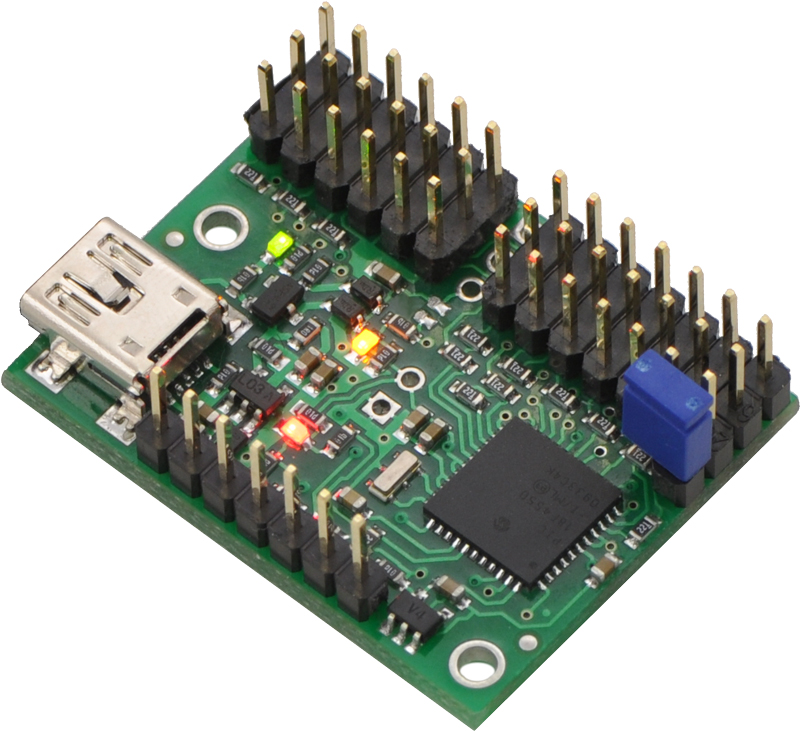
\includegraphics[width=0.7\columnwidth]{../images/maestroServoController.jpg}
			\caption{Quelle: www.pololu.com/product/1352}
		\end{figure}
		\column{0.5\textwidth}
		\begin{figure}
			\centering
			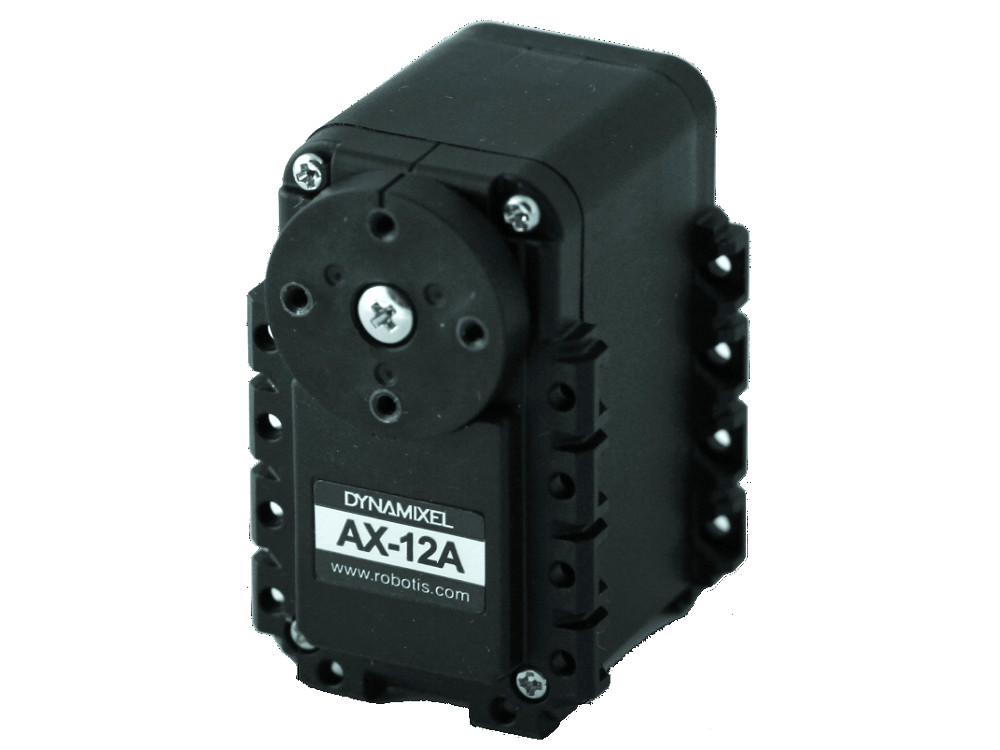
\includegraphics[width=0.9\columnwidth]{../images/dynamixelAX12A.jpg}
			\caption{Quelle: www.eu.diigiit.com/dynamixel-ax-12a}
		\end{figure}
	\end{columns}
	
\end{frame}

\begin{frame}
	\frametitle{Dual Motor Controller}
	
	\begin{columns}[t]
		\column{0.45\textwidth}
		\begin{itemize}
			\item Regelung von 2 DC Motoren
			\item Kommunikation via CAN Bus
			\item Problem: schwache Treiberstufe
		\end{itemize}
		\column{0.45\textwidth}
		%todo Bilder
		Todo Bilder
	\end{columns}
	
\end{frame}

\begin{frame}
	\frametitle{Farbsensor}
	
	\begin{itemize}
		\item Erste Auswahl des Sensors: \textit{Adafruit TCS34725}
		\item Probleme mit I\textsuperscript{2}C
		\item Zweite Auswahl: \textit{Optek OPB780Z}
		\item Frequenzmoduliertes Signal
	\end{itemize}
	
\end{frame}

\begin{frame}
	
	%todo weglassen? (bin mir nicht sicher)
	
	\frametitle{Adapterboard zu Mainboard}
	
	%todo images
	TODO Bilder
	
\end{frame}
  
  %Datenlogger
  \section{Datenlogger}

\begin{frame}
	\frametitle{Hardware}	
	\begin{columns}
		\begin{column}{0.6 \textwidth}
			\begin{itemize}
				\item VDIP1-Board von FTDI
				\item Daten auf USB-Stick speichern und lesen
				\item UART-Schnittstelle
			\end{itemize}
		\end{column}
		\begin{column}{0.4 \textwidth}
			\vspace{-2.8em}
			\begin{figure}[h]
				\centering
				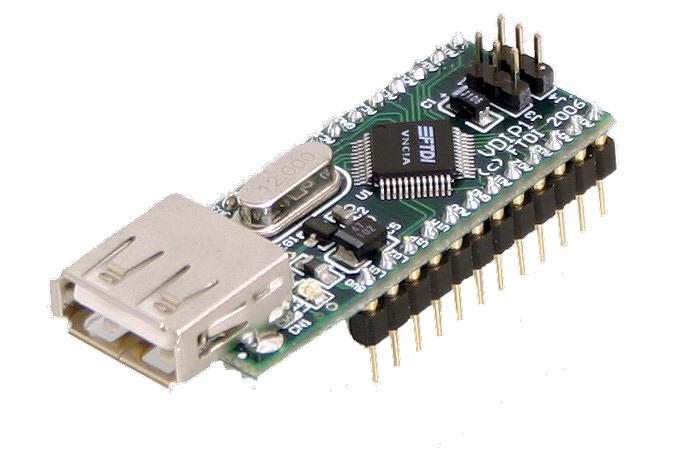
\includegraphics[width = 0.8 \textwidth]{../images/vdip1.jpg}
			\end{figure}
		\end{column}
	\end{columns}
\end{frame}

\begin{frame}
	\frametitle{Software}	
	\begin{itemize}
		\item Steuerung über einfache Befehle
		\item Initialisierung
		\item Ereignisse loggen
		\item Konfigurationsdaten lesen und speichern
	\end{itemize}
\end{frame}

\begin{frame}	
	\frametitle{Probleme}
	\begin{itemize}
		\item Log-Datei wird nicht geschlossen
		\item Absturz des Loggers
	\end{itemize}
	
\end{frame}
  
  %Aufgaben und Strategie
  %\section{Aufgaben und Strategie}

\subsection{Grosser Roboter}

\begin{frame}
	\frametitle{Grosser Roboter}
	\begin{itemize}
		\item Überquerung der Wippe
		\item Aufnahme der \textit{Titanium Ores}
		\item Abschuss der \textit{Titanium Ores} auf dem Spielfeld
		\item Schutz der \textit{Moonbase}
		\item \textit{Funny Action}
	\end{itemize}
\end{frame}

\subsection{Kleiner Roboter}

\begin{frame}
	\frametitle{Kleiner Roboter}
	Aufgaben:
	\begin{itemize}
		\item Modulaufnahme auf dem Feld und aus den Raketen
		\item \textit{Lunar Modules} in \textit{Moonbase} legen
		\item mehrfarbige \textit{Lunar Modules} drehen
		\item \textit{Funny Action}
	\end{itemize}
	\vspace{1em}
	Strategien:
	\begin{itemize}
		\item dem grossen Roboter aus dem Weg gehen
		\item in eigener Spielfeldhälfte bleiben oder beim Gegner Punkte erzielen
	\end{itemize}
\end{frame}
  
  %Wettkampfanalyse
  \section{Wettkampfanalyse}

\begin{frame}
	\frametitle{Homologation}
	
\end{frame}

\begin{frame}
	\frametitle{Schweizermeisterschaft}
	
\end{frame}

\begin{frame}
	\frametitle{Internationale Meisterschaft}
	
\end{frame}
  
  %Rückblick und Fazit
  \section{Fazit}
\begin{frame}
\frametitle{Fazit}

\begin{itemize}
	\item Viele Ziele erreicht
	\item Einiges gelernt
	\item Sinnvolle Aufgabenteilung
	\item Harmonierendes Team
\end{itemize}
\end{frame}    
  
\end{document}
